% Preamble
\documentclass[a4paper,11pt]{article}
\title{}
\author{
    André Cardoso 50\%\\
    andremacardoso@ua.pt\\
    108269\\
    \and
    Tiago Figueiredo 50\%\\
    tiago.a.figueiredo@ua.pt\\
    107263\\
}
\date{09 de Janeiro de 2023}

%packages
\usepackage{graphicx}
\usepackage{xcolor}
\usepackage{listings}
\usepackage[portuguese]{babel}
\usepackage{microtype}
\usepackage{xspace}
\usepackage{url}
\usepackage{csquotes}
\usepackage{lipsum}
\usepackage{array}
\usepackage{multirow}
\usepackage{booktabs}
\usepackage{pdfpages}
\usepackage[
    backend=bibtex,
    style=alphabetic,
    sorting=ynt,
    bibencoding=utf8
]{biblatex}
\addbibresource{Relatorio.bib}

\definecolor{keycolor}{RGB}{172, 42, 42}

\setboolean{@twoside}{false}

\lstdefinestyle{global}{
basicstyle=\ttfamily\scriptsize\color{black!90},%
stringstyle=\itshape\color{magenta},%
showstringspaces=false,%
keywordstyle=\bfseries\color{keycolor},%
commentstyle=\color{blue}\slshape,%
framexleftmargin=1mm,%
backgroundcolor=\color{black!2},%
    }

\lstdefinestyle{makefile}{
otherkeywords={.SUFFIXES},
alsoletter={:},
morekeywords=[1]{SUFFIX, CPP_},
morekeywords=[2]{vasp:,makeparam:,zgemmtest:,dgemmtest:,ffttest:,kpoints:,clean:},
style=global,%
morecomment=[l][commentstyle]{\#},%
emphstyle={\color{vimvert}},%
moredelim=[s][\color{vimvert}]{\$(}{)}%
}

\newcommand{\head}[1]{\textnormal{\textbf{#1}}}
\newcolumntype{P}[1]{>{\centering\arraybackslash}p{#1}}

\definecolor{dkgreen}{rgb}{0,0.6,0}
\definecolor{mauve}{rgb}{0.58,0,0.82}
\definecolor{gray}{rgb}{0.5,0.5,0.5}
\lstset{basicstyle=\ttfamily,
    showstringspaces=false,
    commentstyle=\color{dkgreen},
    keywordstyle=\color{blue},
    columns=flexible,
    basicstyle={\small\ttfamily},
    numbers=left,
    numberstyle=\tiny\color{gray},
    stringstyle=\color{mauve},
    breaklines=true,
    breakatwhitespace=true,
}

% Document
\begin{document}
    \begin{figure}
        \centering
        
\includegraphics[width=0.9\textwidth]{deti2}\label{fig:figure}
    \end{figure}
    \maketitle
    \tableofcontents
    \clearpage


    \section{Introdução}\label{sec:introducao}
Uma word ladder é uma sequência de palavras em que cada palavra difere em uma e só uma letra da palavra anterior.
% Very original
Por exemplo, na língua Portuguesa é possível ir da palavra tudo para a palavra nada em quatro passos.
\emph{$tudo \rightarrow todo \rightarrow nodo \rightarrow nado \rightarrow nada$}.
Como tal para resolver o problema proposto de criar um algoritmo em \emph{C/C++} que permita encontrar foi feita uma implementação de uma \emph{Hash Table} em \emph{C++}, usada depois para permitir a implementação de grafos e do \emph{union find}, tornando possível tal algoritmo.

    \section{Funções Usadas}\label{sec:funcoes-usadas}
    Esta secção contém uma lista, com a respetiva descrição de todas as funções usadas para a criação do algoritmo.

    \subsection{Hash Table}\label{subsec:hash-table}
    Sendo a linguagem de progamação escolhida para a resolução de este problema \emph{C++}, a \emph{Hash table} foi implementada através de duas classes, uma que contém os parâmetros de cada nó da \emph{Hash Table}, e uma que contém a implementação da \emph{Hash Table}.

    \subsubsection{Constructor}
    O construtor inicializa todas as variáveis da classe quando um objeto do tipo da classe é criado. 
    Começa por definir o tamanho da hash table como sendo 65536, cria um array de ponteiros chamado \emph{words} com o tamanho da tabela. Inicializa também a variável \emph{entries} a 0, a variável \emph{connected\_components} também a 0 e a \emph{variável load\_factor} como sendo 0,75. Define, por fim, todos os elementos do array \emph{words} como sendo ponteiros nullos, o que indica que todos os elementos da tabela estão vazios.

    \subsubsection{Destructor}
O destrutor dá um loop pelo array \emph{words} eliminando cada elemento não nulo, acabando por eliminar o array, no final.
   
    \subsubsection{add}
    Esta função é usada para adicionar uma nova palavra à hash table. A função recebe um único argumento, uma string chamada \emph{word} que representa a palavra a ser adicionada à tabela.

    A função começa chamando a função hash() para obter o índice em que a palavra deve ser inserida.
    Em seguida, verifica se a palavra já está presente na tabela verificando se o elemento no índice calculado não é nulo e se a palavra armazenada nesse elemento é a mesma da palavra a ser adicionada. Se a palavra já estiver presente, a função retorna sem adicionar a palavra à tabela.
    A função, caso a palavra não corresponder a nenhuma já existente, verifica se o número de entradas na tabela mais 1 é maior ou igual ao tamanho da tabela multiplicado pelo fator de carga. Se isso for verdade, significa que a tabela está a ficar cheia e é chamada a função resize() para aumentar o tamanho da tabela.
    Se o elemento no índice calculado for nulo, a função chama a função create() para criar um novo nó com a palavra e a inserir no índice caso contrário, se a palavra armazenada nesse elemento não for a mesma da palavra a ser adicionada, a função entra em um loop while. O loop executa até encontrar um espaço vazio na tabela podendo também parar se a palavra já se encontrar na tabela. Para encontrar o próximo espaço disponível, ele usa \emph{linear probing}.
     Linear probing é uma técnica de resolução de colisões onde o próximo espaço é encontrado incrementando o índice um por um até ser encontrada uma posição vazia.
    Se um espaço vazio for encontrado, a função chama a função create(), finalmente criando um novo nó com a palavra e inserindo-a no índice.

    \subsubsection{get}
    Esta função é utilizada para obter um nó específico dado uma palavra. 
    Ela começa chamando a função \emph{hash} para obter o índice onde a palavra deve ser encontrada. Se o elemento no índice calculado for nulo, a função retorna um \emph{nullptr}, indicando que a palavra não está presente.
    Se o elemento não é nulo, ele verifica se a palavra armazenada é a mesma da palavra que se deseja procurar.
    Se for, a função retorna o endereço desse elemento, caso contrário a função entra num loop while usando linear probing, como na função de cima, para encontrar a palavra ou um espaço vazio. A função retorna o endereço do elemento que coném a palavra, caso este seja encontrado ou \emph{nullptr}.

    \subsubsection{add\_edge}
    Esta função é utilizada para adicionar uma aresta entre dois nós na estrutura de dados que representa um grafo. Ela recebe dois argumentos, "from" e "to", que são ponteiros para os nós entre os quais a aresta será adicionada.
    A função adiciona o nó "to" à lista de adjacência do nó "from" e o nó "from" à lista de adjacência do nó "to", estabelecendo assim a conexão entre eles.
    A função incrementa o contador de arestas em ambos os nós, indicando que eles têm uma aresta adicional, chamando por fim a função g\_union que se encontra descrita abaixo.

    \subsubsection{BFS}
    A função BFS é uma implementação de breadth-first search. Ela começa por percorrer todos os nós e marcando-os como não visitados e sem pais (senão incorre o risco de não funcionar caso outra função que modifique os campos visited e parent já tenha sido executada). Em seguida, a função adiciona o nó "from" a uma fila e marca-o como visitado. A função então entra em um loop enquanto a fila não estiver vazia. Dentro do loop, a função pega o primeiro elemento da fila e verifica se é o nó "to". Se for, a função retorna a profundidade atual. Caso contrário, a função percorre todos os nós adjacentes ao nó atual que ainda não foram visitados, marca-os como visitados e adiciona-os à fila. A profundidade é incrementada a cada iteração do loop. Se a profundidade atual é maior que o valor máximo de profundidade especificado e o valor máximo de profundidade é diferente de 0, a função retorna -1. Se o loop termina e o nó "to" ainda não foi encontrado, a função retorna -1.

    \subsubsection{DFS}
    A função DFS é uma implementação de depth-first search. Ela funciona de maneira semelhante à função BFS, mas usa uma pilha em vez de uma fila. A função marca todos os nós como não visitados e sem pais e adiciona o nó "from" à pilha. A função então entra em um loop enquanto a pilha não estiver vazia. Dentro do loop, a função pega o topo da pilha e verifica se é o nó "to". Se for, a função segue o caminho de volta ao nó "from" contando a profundidade e retorna-a. Caso contrário, a função percorre todos os nós adjacentes ao nó atual que ainda não foram visitados, marca-os como visitados e adiciona-os à pilha. Se o loop termina e o nó "to" ainda não foi encontrado, a função retorna -1.
    
    \subsubsection{list\_connected\_components}
    A função list\_connected\_components é usada para listar todos os nós que fazem parte do mesmo componente conectado de um nó específico dado uma palavra. Ela chama a função get para obter o nó correspondente à palavra fornecida, se ele não for encontrado, a função imprime "Palavra não encontrada" e retorna. Caso contrário, ela chama outra função chamada "find", passando o nó encontrado como argumento, essa função retorna um representante de um conjunto na estrutura de dados union-find. Em seguida, a função percorre todos os nós na tabela hash e adiciona a um vetor de componentes todos os nós cujo representante é o mesmo do nó encontrado anteriormente. Finalmente, a função imprime "Pertencente ao mesmo componente conectado como [palavra fornecida]:" e imprime todas as palavras armazenadas nos nós do vetor de componentes.
    
    \subsubsection{find}
    A função \emph{find} é uma função recursiva que encontra o \emph{representative}  de vértice do grafo, verificando se o vértice atual é o requerido até o encontrar.
    
    \subsubsection{g\_union}
    A função \emph{g\_union}, faz uso da função \emph{find}, para encontrar os representativos das nodes \emph{to} e \emph{from}, tornando por fim, o representativo da node \emph{to} no mesmo do da node \emph{from}. Isto só acontece se os representativos não forem os mesmos.
    
    \subsubsection{hash and unhash}
    A função de hash transforma um inteiro ou através do \emph{operator overloading} disponível do \emph{C++}, uma função com o mesmo nome existe para em vez de um inteiro receber uma string, e através do método \emph{64-bit FNV-1a hash} encodificar a string ou inteiro fornecido de modo a poder ser usado como index da hash table. A função unhash reverte este processo, como seria previsivel


    \subsection{Estatísticas da Hash Table}\label{subsec:estatisticas-da-hash-table}

    \subsubsection{get\_load\_factor e get\_collisions}
   As funções get\_load\_factor e get\_collisions são usadas para obter estatísticas sobre a hash table. A primeira função retorna o fator de carga atual, que é o número de entradas na tabela dividido pelo tamanho da tabela. A segunda função retorna o número de colisões na tabela.
    
    \subsubsection{get\_distribution}
    A função get\_distribution é usada para obter a distribuição de entradas na tabela hash. Ela percorre toda a tabela e adiciona "true" a um vetor de bools, que permite com alguns compiladores guardar o valor em um bit, se uma entrada está presente na posição atual ou "false" se não estiver. A função retorna esse vetor.
    
    \subsection{Estatísticas do Grafo}\label{subsec:estatisticas-do-grafo}
    
    \subsubsection{get\_connected\_components}
    A função get\_connected\_components conta o número de componentes conectados no grafo. Ele percorre a tabela hash e verifica, para cada nó, se é um representante de seu conjunto de união (usando a propriedade representative). Se for, incrementa o contador de componentes. O número de componentes conectados é retornado no final.
    
    \subsubsection{get\_diameter}
    A função get\_diameter calcula o diâmetro do componente conexo. O diâmetro é o caminho maior caminho mais curto entre dois nós do mesmo componente conexo. Começa por percorrer a hash table e chama a função DFS em cada nó, passando o nó atual como início e o nó especificado como parâmetro como destino. A distância retornada pela DFS é comparada com a distância máxima encontrada até agora. Se for maior, atualiza a distância máxima e salva o nó inicial. No final, se print for verdadeiro, imprime o diâmetro e o caminho encontrado.
    
    \subsubsection{get\_diameter\_node}
    A função get\_diameter\_node é semelhante à anterior, mas apenas retorna o nó inicial do caminho com o maior diâmetro.

    \subsection{Outras Funções}\label{subsec:outras-funcoes}

    \subsubsection{longest}
    A função "longest" encontra o diâmetro do componente conexo da palavra dada. Ela faz isso chamando o método get\_diameter() da tabela de hash correspondente ao tamanho da palavra dada.
    
    \subsubsection{connected}
    A função "connected" verifica se as duas palavras dadas são conectadas (se elas diferem apenas por uma letra). Ela faz isso comparando cada letra das palavras uma a uma e verificando se elas são diferentes.
    
    \subsubsection{path\_finder}
    A função "path\_finder" é usada para encontrar o caminho mais curto entre duas palavras no grafo. Ele usa a função BFS para encontrar a distância mais curta entre as duas palavras e imprime o caminho encontrado.
    
    \subsubsection{connected\_components}
A função "connected\_components" encontra todas as palavras que estão conectadas (que diferem apenas por uma letra) à palavra dada. Ela faz isso chamando o método list\_connected\_components() da tabela de hash correspondente ao tamanho da palavra dada.
    
    \section{Resultados}\label{sec:resultados}

	\subsection{Resultados gerais}
	Após a execução do programa, foi verificado que este cumpria os testes impostos como condição para verifiacar o bom funcionamento do algoritmo e da hash table.\\
	Alguns destes testes, incluem processar algumas palavras de cada comprimento para verificar que o bom funcionamento do algoritmo e da hash table enquanto este tamanho aumenta, a verificação de uma \emph{word ladder} conhecida, de \emph{etano} a \emph{sitie}, e a confirmação de que o maior tamanho para chegar à primeira dessas duas palavras é 1135.
	Como descrito nas secções abaixo, o programa foi capaz de executar sem a criação de \emph{memory leaks}, e de com a capacidade de correr num servidor durante um longo período de tempo.\\
	Durante este período, foi capaz de encontar várias \emph{word ladders}, sendo que o seu tamanho se encontra no gráfico abaixo.\\
	\begin{figure}[h]
        \centering
        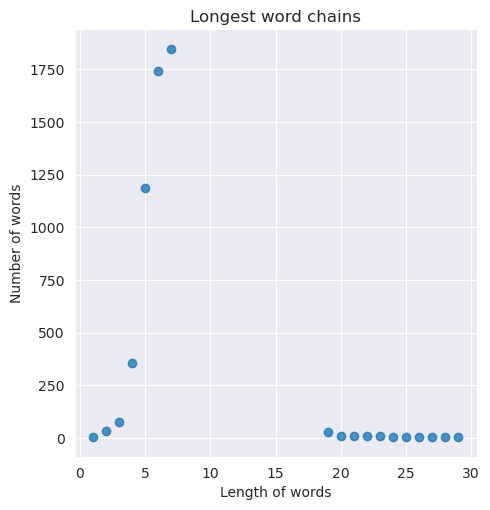
\includegraphics[width=\textwidth]{output_4_1}
        \caption{Comprimento das word ladders}\label{fig:graph-1}
    \end{figure}\\
	Por fim, os dois gráficos seguintes demonstram o de posições ocupadas na hash table, comparados com o número de colisões existentes ao tentar inserir um novo elemento, incluindo a demonstração de que estes valores voltam, como seria esperado, a diminuir, após o aumento da hash table, usando a função \emph{resize}.\\
	\begin{figure}[h]
        \centering
        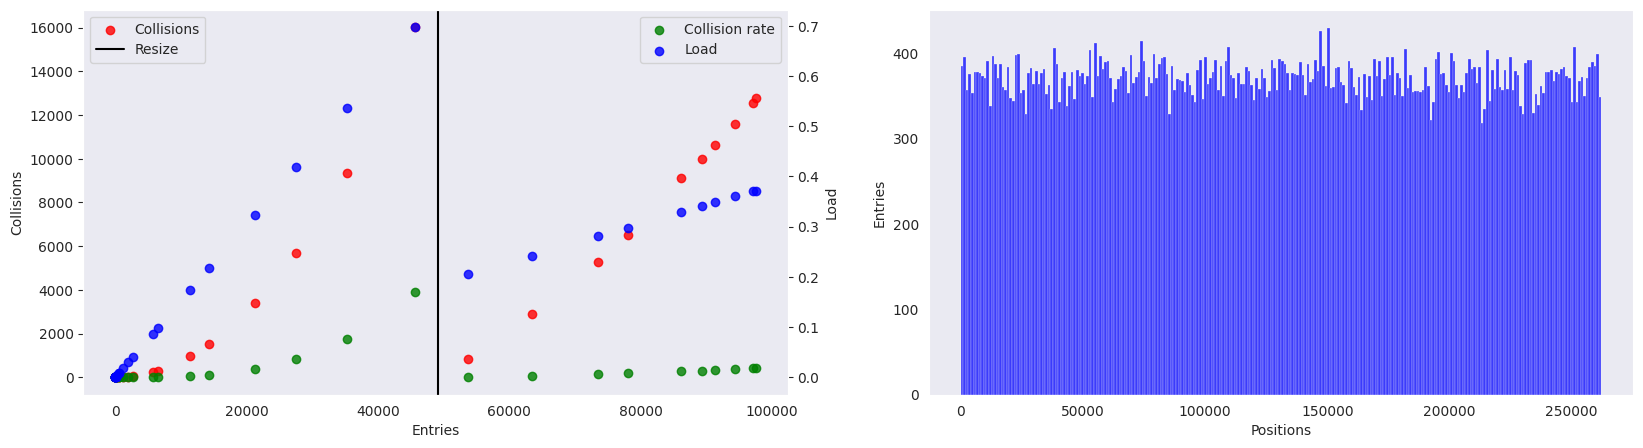
\includegraphics[width=\textwidth]{output_4_0}
        \caption{Comprimento das word ladders}\label{fig:graph-1}
    \end{figure}\\
		
	\subsection{Testes de Memory Leaks}
	Para determinar se o programa tinha \emph{memory leaks}, foi usado o valgrind, com as seguintes opções:\\
	\emph{--leak-check=full \\\
         --show-leak-kinds=all \\\
         --track-origins=yes \\\
         --verbose \\\
         --log-file=valgrind-out.txt \\\
         ./word\_ladder }\\
         Tendo sido obtido o ficheiro de log encontrado no apêndice \emph{valgrind-out.txt}, comprovando que não existem \emph{memory leaks}.
	
	\subsection{Resultados ao fim de 14 dias}
	Devido ao facto de que a lógica principal do programa foi acabada com alguma antecedência, o algoritmo correu com o objetivo de encontrar a maior \emph{ladder} possível, para o dicionário fornecido, para cada tamanho de palavra.
	Infelizmente devido à quantidade de palavras de tamanho superior a oito ou nove letras e inferior a vinte letras, algumas das \emph{ladders} para os comprimentos de palavra nesse intervalo não foram encontrados, tendo a maior sido uma \emph{word ladder} com tamanho 1844 para palavras de tamanho sete.\\ \\
	 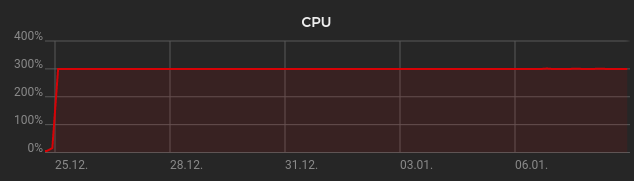
\includegraphics[width=\textwidth]{cpu}\label{fig:figure}\\
	Devido ao uso de todos os threads disponiveis, três núcleos e 6 threads, de um processador \emph{AMD\textsuperscript{TM} Epyc Rome}, o uso do processador manteve-se a 300\% (cada núcleo a 100\%), durante a inteira duração.\\ \\
	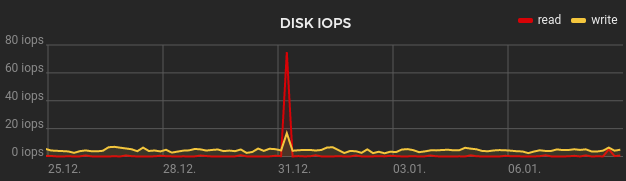
\includegraphics[width=\textwidth]{iops}\label{fig:figure}\\
	O programa também demonstrou um uso residual do disco durante a maioria da sua duração, sendo o pico visivel no gráfico, resultante de um pico no uso de rede enquanto este atualizava, visto que havia mais tarefas a correr no mesmo servidor.\\ \\     
	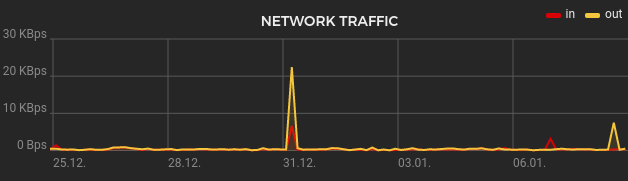
\includegraphics[width=\textwidth]{net}\label{fig:figure}\\    
	Assim sendo, as maiores word ladders encontradas por este programa encontram-se na secção 5.4 do apêndice, sendo que seriam demasiado extensas para se encontrarem nesta descrição.
    \clearpage


    \section{Referências}\label{sec:referencias}~\nocite{aed,cpp,valgrind,fowler,skeeto}
    \printbibliography[
        heading=none,
    ]

    \clearpage


    \section{Apêndice}\label{sec:apendice}
    
    \subsection{word\_ladder.cpp}    
    \begin{lstlisting}[language=c++,label={lst:lstlisting}]
#include <algorithm>
#include <fstream>
#include <iostream>
#include <string>
#include <cmath>
#include <vector>
#include <queue>
#include <stack>
#include <thread>

using namespace std;
#define _max_word_size_ 32

class node {
public:
    node(const string &word) : word(word) {
        parent = nullptr;
        visited = false;
        representative = this;
        vertices = 1;
        edges = 0;
    }

    string word;
    // search relevant data
    node *parent;
    bool visited;
    // graph data structure
    vector<node *> adjacency_list;
    // union-find data structure
    node *representative;
    int vertices;
    int edges;
};

class hashTable {
public:
    unsigned int size;
    node **words;
    unsigned int entries;
    int connected_components;
    double load_factor;

    hashTable() {
        // Makes the dict only need to be resized once.
        size = 65536;
        words = new node *[size];
        entries = 0;
        connected_components = 0;
        load_factor = 0.75;
        for (unsigned int i = 0; i < size; i++) {
            words[i] = nullptr;
        }
    }

    ~hashTable() {
        for (unsigned int i = 0; i < size; i++) {
            if (words[i] != nullptr) {
                delete words[i];
            }
        }
        delete[] words;
    }

    void add(const string &word) {
        unsigned int index = hash(word);
        if (words[index] != nullptr && words[index]->word == word) {
            return;
        }
        if (entries + 1 >= size * load_factor) {
            resize();
        }
        if (words[index] == nullptr) {
            create(index, word);
        } else if (words[index]->word != word) {
            while (words[index] != nullptr && words[index]->word != word) {
                // Linear probing is the fastest way.
                // Probably because it uses the cache more efficiently.
                // And that matters the most when the table is huge and we have memory to spare.
                index = (index + 1) % size;
            }
            create(index, word);
        }
    }

    node *get(const string &word) {
        unsigned int index = hash(word);
        if (words[index] == nullptr) {
            return nullptr;
        }
        if (words[index]->word == word) {
            return words[index];
        }
        while (words[index] != nullptr && words[index]->word != word) {
            index = (index + 1) % size;
        }
        return words[index];
    }

    // graph functions
    void add_edge(node *from, node *to) {
        from->adjacency_list.push_back(to);
        to->adjacency_list.push_back(from);
        from->edges++;
        to->edges++;
        g_union(from, to);
    }

    int BFS(node *from, node *to, int maximum_depth = 0) {
        for (unsigned int i = 0; i < size; i++) {
            if (words[i] != nullptr) {
                words[i]->visited = false;
                words[i]->parent = nullptr;
            }
        }
        queue < node * > q;
        from->visited = true;
        q.push(from);
        int depth = 0;
        while (!q.empty()) {
            int q_size = q.size();
            for (int i = 0; i < q_size; i++) {
                node *current = q.front();
                q.pop();
                if (current == to) {
                    return depth;
                }
                for (size_t j = 0; j < current->adjacency_list.size(); j++) {
                    node *adjacent = current->adjacency_list[j];
                    if (!adjacent->visited) {
                        adjacent->visited = true;
                        adjacent->parent = current;
                        q.push(adjacent);
                    }
                }
            }
            depth++;
            if (depth > maximum_depth && maximum_depth != 0) {
                return -1;
            }
        }
        return -1;
    }

    int DFS(node *from, node *to) {
        for (unsigned int i = 0; i < size; i++) {
            if (words[i] != nullptr) {
                words[i]->visited = false;
                words[i]->parent = nullptr;
            }
        }
        stack < node * > q;
        from->visited = true;
        q.push(from);
        int depth = 0;
        while (!q.empty()) {
            int q_size = q.size();
            for (int i = 0; i < q_size; i++) {
                node *current = q.top();
                q.pop();
                if (current == to) {
                    // god why
                    while (current->parent != nullptr && current != from) {
                        current = current->parent;
                        depth++;
                    }
                    return depth;
                }
                for (size_t j = 0; j < current->adjacency_list.size(); j++) {
                    node *adjacent = current->adjacency_list[j];
                    if (!adjacent->visited) {
                        adjacent->visited = true;
                        adjacent->parent = current;
                        q.push(adjacent);
                    }
                }
            }
        }
        return -1;
    }

    void list_connected_components(const string &word) {
        vector < node * > components;
        node *vertex = get(word);
        if (vertex == nullptr) {
            cout << "Word not found" << endl;
            return;
        }
        node *representative = find(vertex);
        for (unsigned int i = 0; i < size; i++) {
            if (words[i] != nullptr && find(words[i]) == representative) {
                components.push_back(words[i]);
            }
        }
        cout << "Belonging to same connected component as " << word << "are:" << endl;
        for (size_t i = 0; i < components.size(); i++) {
            cout << components[i]->word << "\n";
        }
    }

    // hash table statistics
    double get_load_factor() {
        return (double) entries / size;
    }

    int get_collisions() {
        unsigned int collisions = 0;
        for (unsigned int i = 0; i < size; i++) {
            if (words[i] != nullptr) {
                if (hash(words[i]->word) != i) {
                    collisions++;
                }
            }
        }
        return collisions;
    }

    vector<bool> get_distribution() {
        vector<bool> distribution;
        for (unsigned int i = 0; i < size; i++) {
            if (words[i] != nullptr) {
                distribution.push_back(true);
            } else {
                distribution.push_back(false);
            }
        }
        return distribution;
    }

    // graph statistics
    int get_connected_components() {
        int components = 0;
        for (unsigned int i = 0; i < size; i++) {
            if (words[i] != nullptr) {
                if (words[i]->representative == words[i]) {
                    components++;
                }
            }
        }
        return components;
    }

    int get_diameter(node *n, bool print = true) {
        int diameter = 0;
        node *max = nullptr;
        for (unsigned int i = 0; i < size; i++) {
            if (words[i] != nullptr) {
                if (words[i]->adjacency_list.size() == 0) {
                    continue;
                }
                int distance = DFS(words[i], n);
                if (distance > diameter) {
                    diameter = distance;
                    max = words[i];
                }
            }
        }
        // DFS data is wiped out every run.
        DFS(n, max);
        node *res = max;
        if (res == nullptr) {
            return 0;
        }
        if (print) {
            cout << "Diameter: " << diameter << endl;
            cout << "Path: ";
            if (res == nullptr) {
                cout << "No connected words." << endl;
            }
            while (res->parent != nullptr) {
                cout << res->word << " -> ";
                res = res->parent;
            }
            cout << res->word << endl;
        }

        return diameter;
    }

    node *get_diameter_node(node *n) {
        int diameter = 0;
        node *max = nullptr;
        for (unsigned int i = 0; i < size; i++) {
            if (words[i] != nullptr) {
                int distance = DFS(words[i], n);
                if (distance > diameter) {
                    diameter = distance;
                    max = words[i];
                }
            }
        }
        return max;
    }

private:
    void create(int index, const string &word) {
        entries++;
        connected_components++;
        words[index] = new node(word);
    }

    void resize() {
        // High resize coefficient to reduce resizes, which are expensive.
        int coeff = 4;
        size *= coeff;
        node **new_words = new node *[size];
        for (unsigned int i = 0; i < size; i++) {
            new_words[i] = nullptr;
        }
        for (unsigned int i = 0; i < size / coeff; i++) {
            if (words[i] != nullptr) {
                int index = hash(words[i]->word);
                if (new_words[index] == nullptr) {
                    new_words[index] = words[i];
                } else {
                    while (new_words[index] != nullptr) {
                        index = (index + 1) % size;
                    }
                }
            }
        }
        delete[] words;
        words = new_words;
    }

    node *find(node *vertex) {
        if (vertex->representative != vertex) {
            vertex->representative = find(vertex->representative);
        }
        return vertex->representative;
    }

    void g_union(node *from, node *to) {
        node *from_rep = find(from);
        node *to_rep = find(to);
        if (from_rep != to_rep) {
            to_rep->representative = from_rep;
            connected_components--;
        }
    }

    void print_adjacency_list(node *n) {
        cout << n->word << " -> ";
        for (size_t i = 0; i < n->adjacency_list.size(); i++) {
            cout << n->adjacency_list[i]->word << " ";
        }
        cout << endl;
    }

#define FNV_OFFSET 14695981039346656037UL
#define FNV_PRIME 1099511628211UL

    // Return 64-bit FNV-1a hash for key (NUL-terminated). 
    unsigned int hash(const string &word) {
        uint64_t hash = FNV_OFFSET;
        const char *key = word.c_str();
        for (const char *p = key; *p; p++) {
            hash ^= (uint64_t)(unsigned char)(*p);
            hash *= FNV_PRIME;
        }
        // Ensure hash is adjusted to the size of the table.
        return (size_t)(hash & (uint64_t)(size - 1));
    }

    // https://github.com/skeeto/hash-prospector#three-round-functions
    // Kept for reference.
    unsigned int hash(int x) {
        x ^= x >> 17;
        x *= 0xed5ad4bb;
        x ^= x >> 11;
        x *= 0xac4c1b51;
        x ^= x >> 15;
        x *= 0x31848bab;
        x ^= x >> 14;
        return x;
    }

    unsigned int unhash(int x) {
        x ^= x >> 14 ^ x >> 28;
        x *= 0x32b21703;
        x ^= x >> 15 ^ x >> 30;
        x *= 0x469e0db1;
        x ^= x >> 11 ^ x >> 22;
        x *= 0x79a85073;
        x ^= x >> 17;
        return x;
    }
};

void longest(hashTable **dicts, const string &word) {
    hashTable *dict = dicts[word.size() - 1];
    node *n = dict->get(word);
    cout << "Longest path to " << word << " is " << endl
         << dict->get_diameter(n)
         << " words long." << endl;
    return;
}

bool connected(const string &a, const string &b) {
    if (a.size() != b.size())
        return false;
    bool result = false;
    for (size_t i = 0; i < a.size(); i++) {
        if (a[i] != b[i]) {
            // Only one difference is allowed
            if (result)
                return false;
            result = true;
        }
    }
    return result;
}

void path_finder(hashTable **dicts, const string &start, const string &end) {
    if (start.size() != end.size()) {
        cout << "Cannot compare different sizes." << endl;
        return;
    }
    hashTable *dict = dicts[start.size() - 1];
    cout << "Trying to go from " << start << " to " << end << endl;
    node *from = dict->get(end);
    node *to = dict->get(start);
    if (from == nullptr || to == nullptr) {
        cout << "No path found." << endl;
        return;
    }
    int travelled = dict->BFS(from, to);
    cout << "Travelled " << travelled << " nodes. " << endl;
    node *res = to;
    while (res->parent != nullptr) {
        cout << res->word << " -> ";
        res = res->parent;
    }
    cout << res->word << endl;
}

void connected_components(hashTable **dicts, const string &word) {
    hashTable *dict = dicts[word.size() - 1];
    dict->list_connected_components(word);
}

void end(hashTable **dicts) {
#if defined(_stats_) || defined(_detail_) || defined(_full_)
    ofstream file;
    file.open("stats.txt");
#endif
    for (size_t i = 0; i < _max_word_size_; i++) {
#if defined(_stats_) || defined(_detail_) || defined(_full_)
        file << endl;
        file << "Hash Table for " << i + 1 << " letter words" << endl;
        file << "Size: " << dicts[i]->size << endl;
        file << "Load factor: " << dicts[i]->get_load_factor() << endl;
        file << "Collisions: " << dicts[i]->get_collisions() << endl;
#if defined(_detail_) || defined(_full_)
        vector<bool> distribution = dicts[i]->get_distribution();
        file << "Distribution: " << endl;
        for (size_t j = 0; j < distribution.size(); j++)
        {
            if (distribution[j])
                file << j << " ";
        }
        file << endl;
#endif
#endif
        delete dicts[i];
    }
#if defined(_stats_) || defined(_detail_) || defined(_full_)
    file.close();
#endif
}

void graph_builder(hashTable *dict) {
    int sizes = 0;
    // TODO: Optimize this, O(n^1.5) ish isn't good
    for (size_t i = 0; i < dict->size; i++) {
        node *from = dict->words[i];
        if (from == nullptr)
            continue;
        if (sizes == 0)
            sizes = from->word.size();
        for (size_t j = i + 1; j < dict->size; j++) {
            node *to = dict->words[j];
            if (to == nullptr)
                continue;
            if (connected(from->word, to->word)) {
                dict->add_edge(from, to);
            }
        }
    }
    if (sizes != 0)
        cout << "Processed " << sizes + 1 << " letter words" << endl;
}

void longest_path(hashTable *dict) {
    int largest = 0;
    vector < node * > reprs;
    node *max = nullptr;
    for (unsigned int i = 0; i < dict->size; i++) {
        if (dict->words[i] != nullptr) {
            if (find(reprs.begin(), reprs.end(), dict->words[i]->representative) == reprs.end()) {
                reprs.push_back(dict->words[i]->representative);
                int depth = dict->get_diameter(dict->words[i], false);
                if (depth > largest) {
                    largest = depth;
                    max = dict->words[i];
                }
            }
        }
    }
    node *origin = dict->get_diameter_node(max);
    if (origin == nullptr || max == nullptr) {
        cout << "No path found." << endl;
        return;
    }
    dict->DFS(origin, max);
    node *res = max;
    ofstream file;
    file.open("longest.txt", ios::app);
    file << "Longest path for " << max->word.size() << " letter words" << endl;
    file << "Size: " << largest << endl;
    while (res->parent != nullptr) {
        file << res->word << " -> ";
        res = res->parent;
    }
    file << res->word << endl;
}

int main() {
    setlocale(LC_ALL, ".UTF8");
    hashTable *dicts[_max_word_size_];
    thread threads[_max_word_size_];
    for (size_t i = 0; i < _max_word_size_; i++) {
        dicts[i] = new hashTable;
    }
    ifstream in("wordlist-big-latest.txt");
    if (!in) {
        printf("Error: could not open words file\n");
    }
    string word;
    while (in >> word) {
        int size = word.size();
        dicts[size - 1]->add(word);
    }
    for (int sizes = 0; sizes < _max_word_size_; sizes++) {
        hashTable *dict = dicts[sizes];
        threads[sizes] = thread(graph_builder, dict);
    }
    for (int sizes = 0; sizes < _max_word_size_; sizes++) {
        threads[sizes].join();
    }
    path_finder(dicts, "etano", "sitie");
#ifdef _full_
    ofstream file;
    file.open("longest.txt", ios::trunc);
    file.close();
    for (int sizes = 0; sizes < _max_word_size_; sizes++)
    {
        hashTable *dict = dicts[sizes];
        threads[sizes] = thread(longest_path, dict);
    }
    for (int sizes = 0; sizes < _max_word_size_; sizes++)
    {
        threads[sizes].join();
    }
#endif
    // connected_components(dicts, "belo");
    longest(dicts, "etano");

    // etano and sitia are opposite extremeties of (one of the) main connected component, as they show up in lots of diameters
    end(dicts);
}
    \end{lstlisting}
    
    \subsection{makefile}
     \begin{lstlisting}[style=makefile,label={lst:lstlisting}]
#
# makefile to compile the A.02 assignment (word ladder)
#

clean:
	rm -rf a.out word_ladder *.exe

word_ladder: word_ladder.cpp
	g++ -Wall -Wextra -O3 word_ladder.cpp -o word_ladder -lm -march=native

stats: word_ladder.cpp
	g++ -Wall -Wextra -O3 word_ladder.cpp -o word_ladder -lm -march=native -D_stats_

detail: word_ladder.cpp
	g++ -Wall -Wextra -O3 word_ladder.cpp -o word_ladder -lm -march=native -D_detail_

full: word_ladder.cpp
	g++ -Wall -Wextra -O3 word_ladder.cpp -o word_ladder -lm -march=native -D_full_

debug: word_ladder.cpp
	g++ -Wall -Wextra -O0 -ggdb3 word_ladder.cpp -o word_ladder -lm -march=native -D_full_
\end{lstlisting}

	\subsection{valgrind-out.txt}
	
	\begin{lstlisting}
	==39494== Memcheck, a memory error detector
==39494== Copyright (C) 2002-2022, and GNU GPL'd, by Julian Seward et al.
==39494== Using Valgrind-3.19.0-8d3c8034b8-20220411 and LibVEX; rerun with -h for copyright info
==39494== Command: ./word_ladder
==39494== Parent PID: 1689
==39494== 
--39494-- 
--39494-- Valgrind options:
--39494--    --leak-check=full
--39494--    --show-leak-kinds=all
--39494--    --verbose
--39494--    --log-file=valgrind-out.txt
--39494-- Contents of /proc/version:
--39494--   Linux version 6.1.1-zen1-1-zen (linux-zen@archlinux) (gcc (GCC) 12.2.0, GNU ld (GNU Binutils) 2.39.0) #1 ZEN SMP PREEMPT_DYNAMIC Wed, 21 Dec 2022 22:27:59 +0000
--39494-- 
--39494-- Arch and hwcaps: AMD64, LittleEndian, amd64-cx16-lzcnt-rdtscp-sse3-ssse3-avx-avx2-bmi-f16c-rdrand-rdseed
--39494-- Page sizes: currently 4096, max supported 4096
--39494-- Valgrind library directory: /usr/lib/valgrind
--39494-- Reading syms from /home/mycsina/Projects/Uni/AED/A02/A02/word_ladder
--39494-- Reading syms from /usr/lib/ld-linux-x86-64.so.2
==39494== Downloading debug info for /usr/lib/ld-linux-x86-64.so.2...
--39494--   Considering /home/mycsina/.cache/debuginfod_client/22bd7a2c03d8cfc05ef7092bfae5932223189bc1/debuginfo ..
--39494--   .. CRC is valid
==39494== Successfully downloaded debug file for /usr/lib/ld-linux-x86-64.so.2
--39494-- Reading syms from /usr/lib/valgrind/memcheck-amd64-linux
==39494== Downloading debug info for /usr/lib/valgrind/memcheck-amd64-linux...
==39494== Server query failed: No such file or directory
--39494--    object doesn't have a symbol table
--39494--    object doesn't have a dynamic symbol table
--39494-- Scheduler: using generic scheduler lock implementation.
--39494-- Reading suppressions file: /usr/lib/valgrind/default.supp
==39494== embedded gdbserver: reading from /tmp/vgdb-pipe-from-vgdb-to-39494-by-mycsina-on-???
==39494== embedded gdbserver: writing to   /tmp/vgdb-pipe-to-vgdb-from-39494-by-mycsina-on-???
==39494== embedded gdbserver: shared mem   /tmp/vgdb-pipe-shared-mem-vgdb-39494-by-mycsina-on-???
==39494== 
==39494== TO CONTROL THIS PROCESS USING vgdb (which you probably
==39494== don't want to do, unless you know exactly what you're doing,
==39494== or are doing some strange experiment):
==39494==   /usr/lib/valgrind/../../bin/vgdb --pid=39494 ...command...
==39494== 
==39494== TO DEBUG THIS PROCESS USING GDB: start GDB like this
==39494==   /path/to/gdb ./word_ladder
==39494== and then give GDB the following command
==39494==   target remote | /usr/lib/valgrind/../../bin/vgdb --pid=39494
==39494== --pid is optional if only one valgrind process is running
==39494== 
--39494-- REDIR: 0x40248f0 (ld-linux-x86-64.so.2:strlen) redirected to 0x580bd382 (???)
--39494-- REDIR: 0x40230a0 (ld-linux-x86-64.so.2:index) redirected to 0x580bd39c (???)
--39494-- Reading syms from /usr/lib/valgrind/vgpreload_core-amd64-linux.so
==39494== Downloading debug info for /usr/lib/valgrind/vgpreload_core-amd64-linux.so...
==39494== Server query failed: No such file or directory
--39494--    object doesn't have a symbol table
--39494-- Reading syms from /usr/lib/valgrind/vgpreload_memcheck-amd64-linux.so
==39494== Downloading debug info for /usr/lib/valgrind/vgpreload_memcheck-amd64-linux.so...
==39494== Server query failed: No such file or directory
--39494--    object doesn't have a symbol table
==39494== WARNING: new redirection conflicts with existing -- ignoring it
--39494--     old: 0x040248f0 (strlen              ) R-> (0000.0) 0x580bd382 ???
--39494--     new: 0x040248f0 (strlen              ) R-> (2007.0) 0x04847e20 strlen
--39494-- REDIR: 0x40232d0 (ld-linux-x86-64.so.2:strcmp) redirected to 0x4848d40 (strcmp)
--39494-- REDIR: 0x40224f0 (ld-linux-x86-64.so.2:mempcpy) redirected to 0x484c810 (mempcpy)
--39494-- Reading syms from /usr/lib/libstdc++.so.6.0.30
--39494-- Reading syms from /usr/lib/libm.so.6
==39494== Downloading debug info for /usr/lib/libm.so.6...
--39494--   Considering /home/mycsina/.cache/debuginfod_client/2c8ff1d29b255da5b7371efd5caf57444d622838/debuginfo ..
--39494--   .. CRC is valid
==39494== Successfully downloaded debug file for /usr/lib/libm.so.6
--39494-- Reading syms from /usr/lib/libgcc_s.so.1
--39494-- Reading syms from /usr/lib/libc.so.6
==39494== Downloading debug info for /usr/lib/libc.so.6...
--39494--   Considering /home/mycsina/.cache/debuginfod_client/1e94beb079e278ac4f2c8bce1f53091548ea1584/debuginfo ..
--39494--   .. CRC is valid
==39494== Successfully downloaded debug file for /usr/lib/libc.so.6
==39494== WARNING: new redirection conflicts with existing -- ignoring it
--39494--     old: 0x04c41270 (memalign            ) R-> (1011.0) 0x04847070 memalign
--39494--     new: 0x04c41270 (memalign            ) R-> (1017.0) 0x04847040 aligned_alloc
==39494== WARNING: new redirection conflicts with existing -- ignoring it
--39494--     old: 0x04c41270 (memalign            ) R-> (1011.0) 0x04847070 memalign
--39494--     new: 0x04c41270 (memalign            ) R-> (1017.0) 0x04847010 aligned_alloc
--39494-- REDIR: 0x4c47110 (libc.so.6:strncasecmp) redirected to 0x48361c0 (_vgnU_ifunc_wrapper)
--39494-- REDIR: 0x4c454d0 (libc.so.6:strchrnul) redirected to 0x48361c0 (_vgnU_ifunc_wrapper)
--39494-- REDIR: 0x4c445f0 (libc.so.6:memrchr) redirected to 0x48361c0 (_vgnU_ifunc_wrapper)
--39494-- REDIR: 0x4c43c70 (libc.so.6:memcpy@@GLIBC_2.14) redirected to 0x48361c0 (_vgnU_ifunc_wrapper)
--39494-- REDIR: 0x4c58f70 (libc.so.6:wcslen) redirected to 0x48361c0 (_vgnU_ifunc_wrapper)
--39494-- REDIR: 0x4c5a720 (libc.so.6:wcsnlen) redirected to 0x48361c0 (_vgnU_ifunc_wrapper)
--39494-- REDIR: 0x4c47420 (libc.so.6:strnlen) redirected to 0x48361c0 (_vgnU_ifunc_wrapper)
--39494-- REDIR: 0x4c474b0 (libc.so.6:strpbrk) redirected to 0x48361c0 (_vgnU_ifunc_wrapper)
--39494-- REDIR: 0x4c45560 (libc.so.6:strcmp) redirected to 0x48361c0 (_vgnU_ifunc_wrapper)
--39494-- REDIR: 0x4c44680 (libc.so.6:memset) redirected to 0x48361c0 (_vgnU_ifunc_wrapper)
--39494-- REDIR: 0x4c58d80 (libc.so.6:wcschr) redirected to 0x48361c0 (_vgnU_ifunc_wrapper)
--39494-- REDIR: 0x4c45450 (libc.so.6:index) redirected to 0x48361c0 (_vgnU_ifunc_wrapper)
--39494-- REDIR: 0x4c474e0 (libc.so.6:rindex) redirected to 0x48361c0 (_vgnU_ifunc_wrapper)
--39494-- REDIR: 0x4c58e10 (libc.so.6:wcscmp) redirected to 0x48361c0 (_vgnU_ifunc_wrapper)
--39494-- REDIR: 0x4c448d0 (libc.so.6:stpncpy) redirected to 0x48361c0 (_vgnU_ifunc_wrapper)
--39494-- REDIR: 0x4c593d0 (libc.so.6:wmemchr) redirected to 0x48361c0 (_vgnU_ifunc_wrapper)
--39494-- REDIR: 0x4c472c0 (libc.so.6:strncmp) redirected to 0x48361c0 (_vgnU_ifunc_wrapper)
--39494-- REDIR: 0x4c44940 (libc.so.6:strcasecmp) redirected to 0x48361c0 (_vgnU_ifunc_wrapper)
--39494-- REDIR: 0x4c467d0 (libc.so.6:strcspn) redirected to 0x48361c0 (_vgnU_ifunc_wrapper)
--39494-- REDIR: 0x4c58ea0 (libc.so.6:wcscpy) redirected to 0x48361c0 (_vgnU_ifunc_wrapper)
--39494-- REDIR: 0x4c453d0 (libc.so.6:strcat) redirected to 0x48361c0 (_vgnU_ifunc_wrapper)
--39494-- REDIR: 0x4c471b0 (libc.so.6:strncasecmp_l) redirected to 0x48361c0 (_vgnU_ifunc_wrapper)
--39494-- REDIR: 0x4c43b70 (libc.so.6:bcmp) redirected to 0x48361c0 (_vgnU_ifunc_wrapper)
--39494-- REDIR: 0x4c46750 (libc.so.6:strcpy) redirected to 0x48361c0 (_vgnU_ifunc_wrapper)
--39494-- REDIR: 0x4c449e0 (libc.so.6:strcasecmp_l) redirected to 0x48361c0 (_vgnU_ifunc_wrapper)
--39494-- REDIR: 0x4c47080 (libc.so.6:strlen) redirected to 0x48361c0 (_vgnU_ifunc_wrapper)
--39494-- REDIR: 0x4c47360 (libc.so.6:strncpy) redirected to 0x48361c0 (_vgnU_ifunc_wrapper)
--39494-- REDIR: 0x4c44850 (libc.so.6:stpcpy) redirected to 0x48361c0 (_vgnU_ifunc_wrapper)
--39494-- REDIR: 0x4c443b0 (libc.so.6:memmove) redirected to 0x48361c0 (_vgnU_ifunc_wrapper)
==39494== Preferring higher priority redirection:
--39494--     old: 0x04cfd840 (__memcpy_avx_unalign) R-> (2018.0) 0x0484a040 __memcpy_avx_unaligned_erms
--39494--     new: 0x04cfd840 (__memcpy_avx_unalign) R-> (2018.1) 0x0484b910 memmove
--39494-- REDIR: 0x4c43ae0 (libc.so.6:memchr) redirected to 0x48361c0 (_vgnU_ifunc_wrapper)
--39494-- REDIR: 0x4c476a0 (libc.so.6:strspn) redirected to 0x48361c0 (_vgnU_ifunc_wrapper)
--39494-- REDIR: 0x4c444d0 (libc.so.6:mempcpy) redirected to 0x48361c0 (_vgnU_ifunc_wrapper)
--39494-- REDIR: 0x4c44780 (libc.so.6:rawmemchr) redirected to 0x48361c0 (_vgnU_ifunc_wrapper)
--39494-- REDIR: 0x4c47e50 (libc.so.6:strstr) redirected to 0x48361c0 (_vgnU_ifunc_wrapper)
--39494-- REDIR: 0x4d03930 (libc.so.6:__strrchr_avx2) redirected to 0x4847800 (rindex)
--39494-- REDIR: 0x4c40590 (libc.so.6:malloc) redirected to 0x4841810 (malloc)
--39494-- REDIR: 0x4d00fe0 (libc.so.6:__strlen_avx2) redirected to 0x4847d00 (strlen)
--39494-- REDIR: 0x4cfd0e0 (libc.so.6:__memcmp_avx2_movbe) redirected to 0x484b0c0 (bcmp)
--39494-- REDIR: 0x4d006f0 (libc.so.6:__strcmp_avx2) redirected to 0x4848c40 (strcmp)
--39494-- REDIR: 0x4d026b0 (libc.so.6:__strncmp_avx2) redirected to 0x4848450 (strncmp)
--39494-- REDIR: 0x4d002c0 (libc.so.6:__strchr_avx2) redirected to 0x48479e0 (index)
--39494-- REDIR: 0x4cfce40 (libc.so.6:__memchr_avx2) redirected to 0x4848dc0 (memchr)
--39494-- REDIR: 0x4d00500 (libc.so.6:__strchrnul_avx2) redirected to 0x484c300 (strchrnul)
--39494-- REDIR: 0x4cfd800 (libc.so.6:__mempcpy_avx_unaligned_erms) redirected to 0x484c410 (mempcpy)
--39494-- REDIR: 0x4cfd840 (libc.so.6:__memcpy_avx_unaligned_erms) redirected to 0x484b910 (memmove)
--39494-- REDIR: 0x4c40b30 (libc.so.6:free) redirected to 0x4844200 (free)
--39494-- REDIR: 0x4c40d70 (libc.so.6:realloc) redirected to 0x4846c40 (realloc)
--39494-- REDIR: 0x4cff240 (libc.so.6:__strcasecmp_l_avx2) redirected to 0x4848850 (strcasecmp_l)
--39494-- REDIR: 0x4cfe4f0 (libc.so.6:__stpcpy_avx2) redirected to 0x484b1a0 (stpcpy)
--39494-- REDIR: 0x4911460 (libstdc++.so.6:operator new(unsigned long)) redirected to 0x4841f90 (operator new(unsigned long))
--39494-- REDIR: 0x49114c0 (libstdc++.so.6:operator new[](unsigned long)) redirected to 0x4843270 (operator new[](unsigned long))
--39494-- REDIR: 0x4c41340 (libc.so.6:calloc) redirected to 0x48469c0 (calloc)
--39494-- REDIR: 0x490f6e0 (libstdc++.so.6:operator delete(void*, unsigned long)) redirected to 0x4844af0 (operator delete(void*, unsigned long))
--39494-- REDIR: 0x490f700 (libstdc++.so.6:operator delete[](void*)) redirected to 0x4845a10 (operator delete[](void*))
--39494-- memcheck GC: 1000 nodes, 0 survivors (0.0%)
--39494-- memcheck GC: 1000 nodes, 0 survivors (0.0%)
--39494-- memcheck GC: 1000 nodes, 0 survivors (0.0%)
--39494-- memcheck GC: 1000 nodes, 0 survivors (0.0%)
--39494-- memcheck GC: 1000 nodes, 0 survivors (0.0%)
--39494-- memcheck GC: 1000 nodes, 0 survivors (0.0%)
--39494-- memcheck GC: 1000 nodes, 0 survivors (0.0%)
--39494-- memcheck GC: 1000 nodes, 0 survivors (0.0%)
--39494-- memcheck GC: 1000 nodes, 0 survivors (0.0%)
--39494-- memcheck GC: 1000 nodes, 0 survivors (0.0%)
--39494-- memcheck GC: 1000 nodes, 0 survivors (0.0%)
--39494-- memcheck GC: 1000 nodes, 0 survivors (0.0%)
--39494-- memcheck GC: 1000 nodes, 0 survivors (0.0%)
--39494-- memcheck GC: 1000 nodes, 0 survivors (0.0%)
--39494-- memcheck GC: 1000 nodes, 0 survivors (0.0%)
--39494-- memcheck GC: 1000 nodes, 0 survivors (0.0%)
==39494== 
==39494== HEAP SUMMARY:
==39494==     in use at exit: 0 bytes in 0 blocks
==39494==   total heap usage: 10,831 allocs, 10,831 frees, 17,971,237 bytes allocated
==39494== 
==39494== All heap blocks were freed -- no leaks are possible
==39494== 
==39494== ERROR SUMMARY: 0 errors from 0 contexts (suppressed: 0 from 0)
Footer
	\end{lstlisting}

	\subsection{longest.txt}
	Longest path for 1 letter words
Diameter: 1
v -> x
Longest path for 29 letter words
Diameter: 1
constitucionalizar-vos-íamos -> constitucionalizar-nos-íamos
Longest path for 28 letter words
Diameter: 1
constitucionalizar-te-íamos -> constitucionalizar-me-íamos
Longest path for 2 letter words
Diameter: 30
PS -> PT -> BT -> BE -> CE -> CP -> GP -> GB -> kB -> km -> mm -> ma -> ia -> iv -> xv -> xx -> ex -> eh -> oh -> ou -> tu -> te -> de -> dr -> ar -> as -> vs -> vi -> li -> lo -> no
Longest path for 27 letter words
Diameter: 1
instrumentalizar-vos-íamos -> instrumentalizar-nos-íamos
Longest path for 26 letter words
Diameter: 2
corresponsabilizar-vos-ias -> corresponsabilizar-vos-iam -> corresponsabilizar-nos-iam
Longest path for 3 letter words
Diameter: 74
elo -> eco -> oco -> ovo -> ova -> ola -> ala -> ada -> ade -> ase -> use -> uso -> uno -> ano -> aro -> pro -> pio -> pia -> dia -> diz -> giz -> gim -> rim -> riu -> viu -> vii -> vai -> sai -> sal -> sul -> suo -> duo -> doo -> roo -> roa -> boa -> bom -> som -> sem -> nem -> num -> pum -> pus -> bus -> bis -> tis -> tos -> mos -> mor -> mar -> lar -> las -> ias -> iam -> Sam -> San -> Van -> Vaz -> paz -> pau -> tau -> teu -> meu -> mel -> fel -> fez -> foz -> foi -> fui -> rui -> rei -> dei -> der -> per -> pen
Longest path for 25 letter words
Diameter: 3
transcendentalizar-se-iam -> transcendentalizar-te-iam -> transcendentalizar-te-ias -> transcendentalizar-me-ias
Longest path for 24 letter words
Diameter: 3
contratestemunhar-me-ias -> contratestemunhar-te-ias -> contratestemunhar-te-iam -> contratestemunhar-se-iam
Longest path for 4 letter words
Diameter: 353
sras -> eras -> eram -> iram -> irem -> ires -> ores -> oves -> ovem -> ovam -> oval -> oral -> orai -> trai -> traz -> truz -> cruz -> crua -> frua -> flua -> alua -> alue -> alie -> avie -> avir -> agir -> agiu -> adiu -> adia -> afia -> afta -> apta -> apto -> alto -> alho -> olho -> olmo -> elmo -> ermo -> armo -> arfo -> arfe -> arpe -> arpa -> area -> arei -> grei -> geei -> geai -> ceai -> cear -> tear -> toar -> soar -> suar -> suor -> suou -> soou -> coou -> ceou -> geou -> grou -> arou -> aros -> atos -> ator -> atar -> atam -> adam -> adem -> ades -> ales -> alas -> asas -> asai -> usai -> usam -> usem -> unem -> unes -> unis -> unia -> unha -> unhe -> unge -> urge -> urre -> urra -> urda -> urdo -> urjo -> unjo -> anjo -> ando -> anda -> anca -> inca -> isca -> isco -> asco -> asso -> osso -> ouso -> ougo -> jugo -> jogo -> joga -> ioga -> ioda -> iode -> rode -> rodo -> lodo -> ledo -> vedo -> vejo -> veja -> reja -> ruja -> ruma -> duma -> duna -> puna -> pune -> pule -> pile -> pire -> tire -> tive -> uive -> uivo -> vivo -> viva -> vila -> dila -> dilo -> digo -> ligo -> limo -> cimo -> cima -> cita -> cite -> dite -> dine -> fine -> fino -> nino -> nono -> novo -> nove -> nave -> cave -> cape -> tape -> taxe -> taxa -> tara -> para -> papa -> papo -> pado -> gado -> gajo -> gaja -> gafa -> rafa -> raia -> Gaia -> Gaza -> vaza -> vasa -> vaso -> raso -> ralo -> Palo -> Pato -> nato -> nata -> nada -> cada -> ceda -> cena -> lena -> lona -> loja -> boja -> boje -> bote -> pote -> pose -> cose -> come -> dome -> dobe -> dobo -> bobo -> boio -> bois -> dois -> does -> coes -> coei -> voei -> voem -> moem -> miem -> mies -> fies -> fiei -> piei -> piai -> piam -> liam -> lias -> luas -> ruas -> ruis -> ruim -> ruem -> suem -> suei -> subi -> suba -> juba -> jura -> lura -> lusa -> musa -> mesa -> mexa -> mexo -> nexo -> nego -> sego -> sega -> saga -> sala -> sola -> solo -> tolo -> toro -> moro -> miro -> mira -> miga -> figa -> fixa -> rixa -> roxa -> rosa -> Rosa -> Roma -> toma -> tema -> teme -> leme -> lume -> lute -> luto -> luxo -> laxo -> lavo -> lava -> lama -> mama -> mana -> mane -> mate -> mete -> mede -> fede -> fedi -> feri -> fera -> feia -> feio -> geio -> gero -> zero -> zelo -> pelo -> peco -> pico -> pica -> pisa -> sisa -> siso -> biso -> bise -> base -> bafe -> bafo -> bano -> bani -> bali -> dali -> deli -> devi -> revi -> regi -> rege -> ruge -> muge -> mugi -> muni -> muno -> huno -> humo -> sumo -> sujo -> pujo -> pojo -> pomo -> gomo -> goto -> gota -> dota -> dopa -> copa -> coca -> coco -> foco -> fofo -> fofa -> mofa -> mofe -> mole -> fole -> fale -> gale -> gele -> gela -> nela -> nula -> fula -> fulo -> furo -> faro -> saro -> sare -> vare -> vaie -> vais -> cais -> caio -> cabo -> cubo -> tubo -> tufo -> tifo -> rifo -> rife -> rime
Longest path for 23 letter words
Diameter: 8
desconstitucionalizarei -> desconstitucionalizarem -> desconstitucionalizaram -> desconstitucionalizavam -> desconstitucionalizavas -> desconstitucionalizadas -> desconstitucionalizados -> desconstitucionalizamos -> desconstitucionalizemos
Longest path for 22 letter words
Diameter: 6
desgovernamentalizavam -> desgovernamentalizaram -> desgovernamentalizaras -> desgovernamentalizadas -> desgovernamentalizados -> desgovernamentalizamos -> desgovernamentalizemos
Longest path for 5 letter words
Diameter: 1187
enche -> inche -> incha -> incra -> intra -> entra -> extra -> exara -> exata -> exato -> exalo -> exulo -> exumo -> eximo -> exibo -> exibe -> exile -> exila -> axila -> afila -> afifa -> afife -> afine -> afins -> afias -> aftas -> altas -> altar -> aliar -> adiar -> odiar -> opiar -> opias -> opies -> optes -> optem -> ontem -> untem -> unhem -> unhei -> unhai -> unhar -> untar -> untas -> unias -> uniam -> unjam -> urjam -> urram -> urras -> erras -> eiras -> liras -> lidas -> lidam -> limam -> limai -> ligai -> ligar -> migar -> migam -> mijam -> mujam -> sujam -> subam -> cubam -> cubas -> cujas -> fujas -> fumas -> fumes -> gumes -> guies -> guiem -> geiem -> gemem -> remem -> regem -> reger -> reter -> meter -> metem -> matem -> macem -> maces -> mames -> mamei -> mimei -> rimei -> ripei -> ripem -> rixem -> rixam -> riram -> piram -> pilam -> pilai -> pilei -> pisei -> pisem -> sisem -> sises -> bises -> bases -> banes -> banis -> bania -> banda -> panda -> panca -> manca -> mansa -> massa -> mossa -> mosse -> misse -> misso -> misto -> mosto -> rosto -> rasto -> fasto -> facto -> pacto -> parto -> parlo -> parla -> parva -> larva -> larga -> largo -> cargo -> carpo -> zarpo -> zarpa -> farpa -> farta -> farte -> falte -> falhe -> talhe -> telhe -> telha -> tolha -> solha -> solva -> solve -> salve -> salvo -> salgo -> salga -> salta -> Malta -> Malva -> valva -> valsa -> falsa -> falia -> faliu -> baliu -> balir -> bulir -> bulia -> bulha -> bulhe -> bolhe -> bolho -> rolho -> rilho -> filho -> filha -> milha -> minha -> vinha -> vinda -> finda -> findo -> finco -> cinco -> cisco -> risco -> risca -> rasca -> basca -> basco -> tasco -> talco -> palco -> polco -> poluo -> polua -> polia -> polis -> polos -> povos -> novos -> novas -> noras -> foras -> foram -> focam -> tocam -> togam -> togar -> vogar -> vogas -> jogas -> jogai -> rogai -> regai -> recai -> pecai -> pejai -> pejar -> penar -> penal -> renal -> retal -> fetal -> fatal -> faval -> favas -> facas -> lacas -> lamas -> damas -> dadas -> dados -> danos -> panos -> pinos -> sinos -> sidos -> ridos -> ricos -> bicos -> bicas -> bicai -> bisai -> bisar -> pisar -> posar -> posas -> cosas -> cosam -> cosem -> comem -> comei -> somei -> somai -> domai -> domam -> dotam -> datam -> batam -> bagam -> bagar -> pagar -> pagas -> gagas -> gigas -> digas -> dilas -> delas -> devas -> deves -> dever -> devir -> revir -> reviu -> remiu -> remia -> regia -> regra -> regre -> regue -> legue -> ligue -> migue -> migre -> mitre -> nitre -> nitro -> litro -> livro -> livra -> lavra -> lacra -> lacro -> ladro -> ladre -> padre -> podre -> pobre -> dobre -> dobra -> doera -> moera -> moela -> goela -> grela -> grega -> grego -> prego -> predo -> prado -> orado -> ovado -> ovada -> ovava -> orava -> crava -> ceava -> reava -> reavo -> reato -> meato -> meado -> miado -> miada -> piada -> piava -> fiava -> fiara -> tiara -> toara -> soara -> sofra -> sofre -> cofre -> cofie -> cofio -> copio -> copia -> copra -> coira -> coiro -> doiro -> doido -> doida -> doada -> coada -> corda -> coroa -> coroo -> corvo -> sorvo -> sirvo -> sirva -> sirza -> cirza -> cirze -> cinze -> cinde -> cindi -> cingi -> tingi -> tinge -> finge -> finte -> fonte -> monte -> monge -> longe -> longo -> gongo -> gingo -> mingo -> mango -> manjo -> ranjo -> ranho -> ganho -> ganso -> tanso -> tarso -> tarjo -> sarjo -> sarja -> surja -> surra -> burra -> birra -> birro -> mirro -> murro -> curro -> curso -> cursa -> curta -> culta -> culpa -> culpe -> cuspe -> custe -> suste -> susto -> surto -> surti -> sorti -> sorte -> norte -> noite -> coite -> coice -> foice -> force -> forco -> forno -> torno -> terno -> termo -> teimo -> teixo -> deixo -> dei-o -> dei-a -> deu-a -> dou-a -> dou-o -> douto -> couto -> chuto -> chupo -> chupe -> chape -> chame -> chamo -> clamo -> clama -> clima -> clica -> clico -> clivo -> crivo -> privo -> priva -> prova -> trova -> trovo -> trono -> trino -> trine -> urine -> urina -> crina -> china -> chita -> chata -> chaga -> chega -> checa -> cueca -> sueca -> sueva -> suava -> suada -> suado -> soado -> soldo -> solto -> volto -> vulto -> multo -> muito -> quito -> quita -> quina -> quine -> guine -> guise -> guiso -> griso -> iriso -> irisa -> frisa -> frita -> frota -> brota -> brote -> trote -> troce -> trace -> trave -> grave -> gravo -> grano -> grana -> grada -> arada -> asada -> asado -> atado -> ataco -> ataca -> atava -> amava -> amova -> amola -> atola -> atolo -> afolo -> aforo -> afora -> agora -> agira -> agita -> apita -> apipa -> apipo -> apupo -> apuro -> aparo -> avaro -> avara -> alara -> alapa -> alapo -> alago -> alego -> adego -> adega -> adeja -> areja -> arejo -> brejo -> breio -> breia -> creia -> crema -> creme -> treme -> tremo -> trepo -> trepa -> tripa -> gripa -> gripe -> grite -> grete -> frete -> freto -> ereto -> ereta -> preta -> prata -> trata -> traja -> trajo -> trago -> drago -> draga -> Braga -> Brama -> brama -> bramo -> aramo -> arame -> afame -> afama -> acama -> acaba -> acabe -> acate -> acato -> acaso -> acuso -> acuse -> acure -> ature -> atire -> ative -> ativo -> atino -> atina -> atida -> avida -> avido -> amido -> amigo -> amiga -> amiba -> ameba -> amena -> ameno -> ameio -> ateio -> ateie -> apeie -> apeia -> apela -> anela -> anele -> anile -> anise -> aniso -> anoso -> anojo -> anoja -> anota -> azota -> azote -> adote -> adoto -> adito -> edito -> edita -> emita -> emite -> elite -> elide -> elude -> ilude -> iludo -> aludo -> aludi -> aluei -> aguei -> aguai -> aguar -> atuar -> atuas -> atues -> atuem -> anuem -> andem -> andam -> ardam -> arpam -> arpem -> armem -> armei -> armai -> armar -> arfar -> arfas -> areas -> arees -> artes -> antes -> entes -> estes -> esses -> asses -> assas -> ansas -> ancas -> incas -> iscas -> iscos -> ascos -> arcos -> arcou -> areou -> ateou -> atuou -> aluou -> aluiu -> fluiu -> fluir -> fruir -> fruis -> freis -> ireis -> irais -> trais -> toais -> doais -> doeis -> coeis -> ceeis -> ceais -> geais -> geris -> geriu -> gerou -> gemou -> gamou -> gabou -> babou -> bafou -> safou -> sacou -> secou -> secos -> selos -> zelos -> zelou -> melou -> meloa -> melra -> melro -> medro -> cedro -> cetro -> cetra -> letra -> leira -> leiga -> veiga -> verga -> veria -> viria -> viril -> viral -> virar -> oirar -> obrar -> obrai -> obrei -> obrem -> abrem -> abres -> abris -> abria -> arria -> ardia -> urdia -> urdir -> urgir -> ungir -> ungis -> unges -> urges -> urdes -> irdes -> iodes -> iodas -> iodar -> rodar -> radar -> fadar -> fadam -> nadam -> nadem -> nades -> fades -> fales -> falem -> fazem -> jazem -> jazam -> jazas -> vazas -> vasas -> rasas -> raias -> raios -> rabos -> nabos -> natos -> gatos -> galos -> talos -> talas -> balas -> bafas -> bufas -> bufam -> bufem -> bufei -> rufei -> rufai -> tufai -> tufar -> lufar -> lunar -> lanar -> danar -> dinar -> ninar -> ninam -> tinam -> tinas -> tonas -> topas -> topes -> tomes -> domes -> dotes -> notes -> notei -> rotei -> rotem -> lotem -> lutem -> luzem -> luzam -> luxam -> luxai -> luxei -> lixei -> lixes -> lixos -> lixou -> fixou -> ficou -> nicou -> ninou -> minou -> mimou -> mimos -> vimos -> vemos -> remos -> regos -> cegos -> cepos -> copos -> cocos -> cacos -> cavos -> cavou -> lavou -> levou -> nevou -> negou -> pegou -> pejou -> pojou -> posou -> pisou -> pilou -> pulou -> puxou -> puxos -> puxes -> punes -> munes -> munas -> mulas -> pulas -> putas -> lutas -> lutos -> lusos -> fusos -> furos -> furou -> murou -> mudou -> mudos -> modos -> godos -> gomos -> somos -> somou -> domou -> dotou -> rotou -> rolou -> ralou -> rapou -> tapou -> tarou -> torou -> toros -> tiros -> tifos -> tufos -> tufou -> rufou -> rumou -> rumor -> tumor -> temor -> tenor -> menor -> menos -> fenos -> fetos -> tetos -> tesos -> tesas -> temas -> gemas -> geias -> feias -> frias -> irias -> iriam -> triam -> troam -> troas -> troes -> tries -> triei -> criei -> chiei -> chies -> chias -> chiam -> caiam -> caiai -> vaiai -> vaiei -> raiei -> rasei -> rasem -> rafem -> rafes -> rifes -> rifas -> rimas -> rimar -> remar -> rezar -> rezam -> reiam -> leiam -> levam -> lavam -> lavem -> lavei -> cavei -> catei -> cates -> cites -> fites -> fitas -> fitar -> filar -> folar -> bolar -> botar -> cotar -> corar -> corai -> gorai -> gorei -> gozei -> gozem -> gizem -> gizes -> gazes -> gabes -> gabem -> babem -> bebem -> bebam -> bebas -> Tebas -> Texas -> mexas -> mexam -> vexam -> vetam -> vetas -> vedas -> vedar -> velar -> valar -> valam -> galam -> galai -> galei -> gelei -> selei -> sedei -> cedei -> cedem -> fedem -> fodem -> modem -> movem -> sovem -> soves -> sobes -> sebes -> seres -> leres -> leses -> peses -> pedes -> redes -> reles -> veles -> velem -> pelem -> pulem -> pujem -> pujei -> pojei -> podei -> podai -> podal -> modal -> moral -> mural -> murar -> jurar -> juras -> jures -> cures -> curei -> durei -> durem -> murem -> mirem -> minem -> finem -> finei -> fanei -> panei -> panem -> papem -> tapem -> tapam -> rapam -> rapai -> ratai -> matai -> matas -> motas -> mocas -> socas -> socar -> secar -> segar -> segas -> sugas -> rugas -> rugis -> rugir -> augir -> augiu -> mugiu -> mugia -> munia -> punia -> punha -> cunha -> cunho -> junho -> junco -> junca -> junta -> janta -> jante -> cante -> canto -> banto -> bento -> lento -> lenho -> tenho -> tendo -> tende -> vende -> verde -> perde -> perda -> perua -> perus -> peras -> ceras -> caras -> canas -> sanas -> sanam -> saram -> sarai -> tarai -> tirai -> tirei -> virei -> verei -> verti -> verto -> certo -> cesto -> cesta -> lesta -> lesma -> lesme -> lesse -> lasse -> passe -> passo -> posso -> poiso -> poise -> pouse -> pousa -> poupa -> pompa -> pomba -> bomba -> bumba -> zumba -> zumbe -> zombe -> tombe -> tombo -> lombo -> lambo -> lambe -> sambe -> samba -> saiba -> caiba -> caixa -> baixa -> baixo -> faixo -> faixe -> feixe -> feire -> febre -> febra -> ferra -> terra -> tenra -> tensa -> densa -> denso -> senso -> sonso -> sonho -> ponho -> pondo -> ponde -> ronde -> ronda -> sonda -> senda -> senta -> sente -> rente -> reste -> riste -> diste -> dista -> pista -> posta -> porta -> porra -> zorra -> zorro -> jorro -> jarro -> varro -> vario -> varie -> carie -> caria -> cabia -> sabia -> sadia -> sadio -> sacio -> sacie -> sache -> sacha -> tacha -> tacho -> macho -> malho -> calho -> calha -> calda -> calde -> balde -> baldo -> bardo -> bordo -> borde -> borre -> barre -> garre -> garra -> marra -> magra -> magoa -> lagoa -> lagos -> logos -> lobos -> lobas -> lojas -> bojas -> bojes -> bofes -> mofes -> mores -> pores -> pares -> tares
Longest path for 21 letter words
Diameter: 7
petrificar-vos-íamos -> petrificar-nos-íamos -> putrificar-nos-íamos -> nutrificar-nos-íamos -> nutrificar-vos-íamos -> nitrificar-vos-íamos -> vitrificar-vos-íamos -> vitrificar-nos-íamos
Longest path for 6 letter words
Diameter: 1741
enviei -> enfiei -> enfeei -> enfeai -> enfear -> enfiar -> enfiam -> enviam -> envias -> envios -> enviou -> enfiou -> enfeou -> enteou -> entoou -> enjoou -> enjoos -> enjoes -> entoes -> entoas -> entoai -> entrai -> extrai -> extras -> exaras -> exaram -> exarem -> exalem -> exales -> exules -> emules -> emulas -> emulam -> exulam -> exular -> exilar -> axilar -> asilar -> asilas -> afilas -> afixas -> afixos -> afixou -> afinou -> afanou -> abanou -> abonou -> abonos -> abones -> abobes -> adobes -> adubes -> adules -> anules -> anulas -> anelas -> anelai -> anexai -> anexam -> anexem -> anexes -> anexos -> anexou -> anelou -> anilou -> animou -> amimou -> amigou -> amigos -> amidos -> adidos -> adidas -> aditas -> aditar -> agitar -> agitam -> apitam -> apipam -> apipar -> apupar -> apupas -> apupos -> apupou -> apipou -> apitou -> apitos -> apites -> apipes -> apipei -> apupei -> apurei -> acurei -> acures -> amures -> amurem -> aturem -> atarem -> alarem -> alares -> arares -> arades -> brades -> brames -> bramis -> bramiu -> bramou -> tramou -> travou -> cravou -> crivou -> privou -> provou -> prosou -> presou -> presos -> preses -> predes -> credes -> crepes -> trepes -> trepei -> trepai -> tremai -> tremas -> cremas -> creias -> cheias -> chegas -> chegai -> chagai -> chagar -> chamar -> chamam -> clamam -> clamem -> clames -> claves -> clives -> crives -> crises -> irises -> irisei -> irisai -> irisar -> frisar -> frisam -> fresam -> fresai -> presai -> predai -> predar -> pregar -> pregas -> pragas -> dragas -> dragam -> tragam -> tragai -> trajai -> trajei -> tracei -> tracem -> trazem -> trazes -> traves -> troves -> trovas -> provas -> provar -> prover -> provem -> provim -> provia -> previa -> previu -> premiu -> premir -> fremir -> fremis -> fremes -> fremem -> cremem -> cremei -> premei -> primei -> privei -> privai -> privam -> crivam -> crivar -> clivar -> clicar -> clicas -> plicas -> placas -> planas -> planos -> pianos -> piados -> fiados -> fiamos -> fiemos -> viemos -> voemos -> coemos -> coamos -> coados -> zoados -> zoadas -> voadas -> veadas -> meadas -> meados -> meatos -> beatos -> boatos -> boatou -> bostou -> bastou -> pastou -> passou -> pausou -> pousou -> poisou -> poisos -> coisos -> coisas -> coimas -> colmas -> colmar -> calmar -> palmar -> palmam -> pasmam -> pasmai -> pasmei -> pasmes -> palmes -> palpes -> palpos -> palpou -> palmou -> calmou -> calmos -> caldos -> saldos -> saldou -> salgou -> galgou -> galeou -> goleou -> golfou -> golfos -> golfas -> golfai -> golfei -> goleei -> galeei -> baleei -> baseei -> faseei -> faseai -> gaseai -> gasear -> basear -> balear -> baldar -> baldai -> saldai -> soldai -> soltai -> voltai -> voltam -> voltem -> volvem -> volveu -> solveu -> sorveu -> sorves -> torves -> torces -> torcem -> torrem -> borrem -> berrem -> serrem -> seriem -> series -> sedies -> sediei -> mediei -> medrei -> medres -> madres -> padres -> podres -> pobres -> cobres -> coeres -> roeres -> roerem -> moerem -> moeram -> moeras -> moelas -> goelas -> goelam -> grelam -> gretam -> gretem -> gretes -> greles -> grelos -> grilos -> grifos -> grafos -> grafou -> gradou -> aradou -> arador -> atador -> atados -> atamos -> aramos -> iramos -> irados -> iradas -> iraras -> oraras -> oravas -> aravas -> amavas -> amovas -> amoras -> adoras -> adorai -> adotai -> anotai -> anatai -> anafai -> anafar -> abafar -> abalar -> abalas -> abatas -> abatam -> acatam -> acatem -> anatem -> anates -> anafes -> abafes -> abafem -> abanem -> abanei -> abanai -> afanai -> afanam -> afagam -> apagam -> apagai -> apegai -> apegar -> adegar -> adegas -> alegas -> alagas -> aladas -> asadas -> usadas -> usavas -> usavam -> usaram -> usarem -> usarei -> asarei -> afarei -> aforei -> aforem -> aporem -> apoiem -> apoiam -> apeiam -> apeias -> apenas -> acenas -> acenai -> acendi -> acenda -> agenda -> agendo -> atendo -> atando -> amando -> amanho -> amanha -> amansa -> amassa -> amossa -> amosso -> acosso -> acosse -> acesse -> atesse -> atasse -> arasse -> irasse -> iraste -> traste -> triste -> trista -> crista -> crispa -> crespa -> crespo -> cresto -> presto -> presta -> fresta -> fresca -> fresco -> frasco -> franco -> tranco -> trinco -> brinco -> brinca -> brinda -> brinde -> blinde -> alinde -> alinhe -> alinho -> azinho -> azinha -> avinha -> avinca -> avinco -> avindo -> aviado -> adiado -> adiada -> aliada -> alhada -> achada -> achara -> aclara -> aclama -> aclamo -> aclimo -> aclime -> acoime -> acoima -> acoita -> amoita -> amonta -> aponta -> aponte -> aporte -> aborte -> aborde -> abordo -> acordo -> acorda -> acorra -> acorre -> aforre -> aferre -> aferra -> aferia -> aderia -> adiria -> aviria -> avaria -> amaria -> amarra -> amarro -> amargo -> alargo -> alarga -> alarma -> alarme -> alarde -> atarde -> aturde -> aturdo -> atuado -> aguado -> aguada -> aguava -> agrava -> agrafa -> agrafe -> agrade -> agride -> agrido -> abrido -> abrida -> abrira -> abeira -> abeiro -> aberro -> aberto -> aberta -> alerta -> alerte -> aleite -> aleito -> alento -> avento -> aventa -> atenta -> atente -> atinte -> atinge -> atingi -> atinai -> atinar -> ativar -> ativer -> ativei -> avivei -> avives -> avivas -> avisas -> anisas -> anisar -> animar -> animai -> amimai -> amimei -> amimes -> animes -> animem -> anilem -> anilei -> anisei -> alisei -> alises -> alijes -> alojes -> alojem -> alojam -> anojam -> anojas -> enojas -> enojai -> enojei -> anojei -> amojei -> amolei -> amolai -> amolam -> atolam -> atolem -> atoles -> atores -> ateres -> aterei -> iterei -> iterai -> iteram -> ateram -> atiram -> atiras -> aturas -> aturai -> amurai -> amarai -> amaram -> azaram -> azarar -> aparar -> aparas -> aparos -> aparou -> amarou -> amurou -> acurou -> acusou -> abusou -> abusos -> abuses -> abusem -> acusem -> acusam -> acusas -> acudas -> ajudas -> ajudam -> aludam -> iludam -> iludem -> eludem -> eludes -> eludis -> aludis -> alueis -> amueis -> amuais -> anuais -> andais -> ardais -> ardeis -> areeis -> apeeis -> apeais -> ateais -> atrais -> abrais -> obrais -> ourais -> jurais -> jureis -> fureis -> fumeis -> fumais -> sumais -> sujais -> sujeis -> pujeis -> puxeis -> pixeis -> pileis -> fileis -> filais -> ficais -> bicais -> bisais -> cisais -> ciseis -> viseis -> viveis -> vivais -> vitais -> vetais -> metais -> mexais -> mexeis -> meleis -> releis -> reveis -> deveis -> devais -> demais -> temais -> temeis -> gemeis -> gameis -> gamais -> gabais -> babais -> bagais -> pagais -> papais -> tapais -> tarais -> sarais -> sacais -> socais -> vocais -> vogais -> togais -> tonais -> toneis -> topeis -> dopeis -> dobeis -> dobais -> dosais -> rosais -> rotais -> ratais -> latais -> lutais -> luxais -> lixais -> rixais -> rimais -> rimeis -> mimeis -> mijeis -> mijais -> migais -> sigais -> sinais -> ninais -> nineis -> naneis -> faneis -> fadeis -> fedeis -> sedeis -> sedais -> selais -> pelais -> pulais -> punais -> munais -> mungis -> munges -> monges -> montes -> pontes -> pondes -> pordes -> bordes -> bordos -> bardos -> barcos -> marcos -> mancos -> mansos -> tansos -> tangos -> tangou -> tangeu -> tangei -> rangei -> rangem -> rancem -> dancem -> dances -> lances -> lancei -> lanhei -> lanhem -> lanham -> lanhar -> banhar -> banhai -> banzai -> banzam -> baniam -> baliam -> buliam -> bulias -> bulhas -> bulhar -> bilhar -> rilhar -> rilhas -> pilhas -> pilhes -> pilhem -> rilhem -> rilhei -> rolhei -> molhei -> molhes -> folhes -> falhes -> faltes -> faltei -> fartei -> fartai -> fartar -> faltar -> saltar -> saltam -> salgam -> salgas -> salsas -> balsas -> bolsas -> bolsos -> bolsou -> bolhou -> rolhou -> ralhou -> falhou -> faltou -> fartou -> fartos -> factos -> fachos -> fechos -> fechas -> fecham -> ficham -> fichem -> fiches -> biches -> boches -> coches -> cochas -> tochas -> tolhas -> telhas -> telham -> tenham -> renham -> renhas -> senhas -> sonhas -> sonham -> sondam -> rondam -> rondai -> rondei -> mondei -> mordei -> mordem -> moldem -> toldem -> toldes -> soldes -> soltes -> soltos -> soutos -> sou-os -> dou-os -> deu-os -> deu-as -> deusas -> deuses -> reuses -> reusem -> reusam -> reusai -> ressai -> gessai -> gessas -> cessas -> cesses -> cessem -> dessem -> descem -> descei -> descai -> pescai -> pescar -> piscar -> biscar -> biscai -> riscai -> riscam -> discam -> dispam -> dispas -> distas -> mistas -> mistos -> vistos -> vastos -> rastos -> rostos -> gostos -> gestos -> lestos -> leitos -> leitor -> reitor -> reator -> reatou -> restou -> testou -> tentou -> sentou -> sentiu -> sentis -> mentis -> mentia -> meneia -> medeia -> medeio -> mede-o -> medi-o -> medico -> dedico -> dedica -> debica -> debita -> rebita -> recita -> recito -> receto -> recete -> remete -> remate -> remato -> remoto -> remota -> remova -> renova -> renove -> renome -> retome -> retomo -> retoco -> reboco -> reboca -> rebola -> recola -> recoza -> recozo -> recoso -> recose -> recase -> recave -> recavo -> recaio -> recais -> reiais -> leiais -> lesais -> leseis -> peseis -> poseis -> poreis -> moreis -> mofeis -> mofais -> modais -> iodais -> iodeis -> rodeis -> rodeia -> rodeta -> rodete -> rolete -> colete -> colite -> colige -> coliga -> colina -> coluna -> comuna -> comuta -> comuto -> cometo -> coreto -> careto -> cateto -> catito -> catita -> capita -> capina -> cabina -> cabida -> cabido -> sabido -> subido -> sumido -> sumida -> sumira -> sugira -> sugara -> sugava -> sujava -> sujada -> sujado -> sugado -> ougado -> ousado -> ousada -> ousara -> ourara -> curara -> cubara -> cubana -> cubano -> cubado -> jubado -> jurado -> furado -> furada -> murada -> murava -> morava -> gorava -> gozava -> gozara -> gizara -> gizada -> gizado -> girado -> virado -> visado -> bisado -> bisada -> bicada -> bicava -> ficava -> focava -> locava -> locara -> tocara -> tonara -> tonava -> topava -> dopava -> dosava -> dosara -> dobara -> dobada -> lobada -> lobado -> locado -> cocado -> cocada -> cacada -> capada -> capara -> casara -> casava -> caiava -> vaiava -> valava -> falava -> fadava -> fadara -> fanara -> danara -> datara -> ditara -> fitara -> fitada -> fitado -> ditado -> datado -> matado -> matada -> mamada -> mamava -> mimava -> minava -> ninava -> nanava -> panava -> pagava -> pagara -> vagara -> varara -> virara -> virava -> pirava -> pilava -> pelava -> pejava -> pojava -> pojara -> podara -> iodara -> iodada -> iodado -> podado -> posado -> posada -> pomada -> tomada -> tomado -> topado -> tapado -> tarado -> tarada -> talada -> talara -> ralara -> rafara -> rafava -> ratava -> rotava -> notava -> notara -> botara -> botada -> bolada -> bulada -> bufada -> bafada -> babada -> babado -> gabado -> galado -> ralado -> ramado -> ramudo -> rabudo -> rabujo -> rabuje -> rabule -> cabule -> cabula -> cabala -> cavala -> cavalo -> cavado -> cagado -> vagado -> vogado -> votado -> vetado -> velado -> velada -> velara -> gelara -> gerara -> gerira -> ferira -> ferida -> ferido -> fedido -> cedido -> cedida -> medida -> mexida -> mexido -> metido -> detido -> devido -> devida -> decida -> tecida -> temida -> temido -> remido -> relido -> relida -> retida -> retina -> retine -> refine -> refino -> refiro -> refira -> refila -> repila -> repisa -> repesa -> retesa -> retese -> reteve -> releve -> releva -> relega -> delega -> delego -> denego -> renego -> refego -> refugo -> refuto -> reduto -> reduzo -> reluzo -> reluza -> reluta -> relata -> delata -> delate -> debate -> debute -> debuto -> deputo -> depuro -> deparo -> reparo -> repare -> separe -> separa -> secara -> pecara -> pesara -> lesara -> legara -> legada -> regada -> regado -> regalo -> regulo -> regula -> regela -> revela -> revelo -> rebelo -> rabelo -> tabelo -> tabele -> tabefe -> tarefe -> tarefa -> tareca -> careca -> caneca -> caneco -> canelo -> capelo -> capela -> capeia -> mapeia -> mapeio -> mareio -> mareie -> rareie -> rareia -> raleia -> baleia -> baleie -> galeie -> goleie -> goteie -> loteie -> loteis -> coteis -> coceis -> caceis -> caleis -> calais -> valais -> vazais -> vazeis -> vareis -> vereis -> vereia -> sereia -> servia -> servis -> serzis -> cerzis -> cernis -> cernas -> cernam -> cercam -> cercai -> cerrai -> ferrai -> ferrei -> feirei -> feires -> feixes -> deixes -> deixei -> deixai -> deitai -> deitam -> deitem -> dentem -> sentem -> sentei -> ventei -> vencei -> vencem -> vendem -> pendem -> pendam -> pensam -> pensas -> pencas -> percas -> perdas -> herdas -> hordas -> mordas -> mornas -> moinas -> moitas -> muitas -> quitas -> quitam -> quinam -> quinem -> quines -> guines -> guinei -> guisei -> guisem -> guisam -> guisas -> grisas -> brisas -> brigas -> brigai -> britai -> britei -> britem -> brotem -> trotem -> trotam -> trotai -> trocai -> trocar -> brocar -> brocas -> bromas -> brumas -> bruxas -> bruxos -> brutos -> brotos -> brotou -> britou -> fritou -> fritos -> fritas -> frutas -> trutas -> tratas -> tratar -> tramar -> gramar -> granar -> granas -> granes -> granem -> grafem -> grafei -> grafai -> gradai -> gradam -> gravam -> geavam -> geavas -> reavas -> relvas -> relvam -> relvem -> reavem -> reagem -> reages -> reates -> rentes -> lentes -> lenhes -> lenhos -> lenhou -> lanhou -> ganhou -> ganhos -> galhos -> galhas -> malhas -> manhas -> mandas -> mandam -> mangam -> mangar -> mancar -> mancai -> marcai -> marcam -> marram -> garram -> garras -> jarras -> jardas -> sardas -> sarjas -> sarjes -> sarjem -> sarnem -> sornem -> sornei -> tornei -> tornai -> tornar -> torvar -> turvar -> curvar -> curvas -> cursas -> curses -> curtes -> curtos -> certos -> cercos -> circos -> ciscos -> riscos -> riscou -> roscou -> foscou -> forcou -> forrou -> forros -> fornos -> tornos -> turnos -> turbos -> turbas -> turras -> zurras -> zurrai -> surrai -> surram -> supram -> suprem -> soprem -> sopres -> sopros -> soprou -> sobrou -> dobrou -> dourou -> lourou -> louvou -> louvor -> louvar -> louvas -> loucas -> moucas -> moucos -> mouros -> touros -> toiros -> loiros -> loires -> loirei -> doirei -> doarei -> zoarei -> zoarem -> coarem -> coaxem -> coaxei -> coaxai -> coaxas -> coaras -> toaras -> toaram -> voaram -> voavam -> doavam -> doavas -> soavas -> solvas -> solvam -> sorvam -> sirvam -> sirvas -> sirzas -> cirzas -> cirzes -> cirzem -> cinzem -> cindem -> cindes -> cinges -> finges -> fingem -> fintem -> fintei -> fintai -> fincai -> vincai -> vincam -> vingam -> xingam -> xingas -> gingas -> ginjas -> cinjas -> cinjam -> tinjam -> tanjam -> tanjas -> tantas -> santas -> sintas -> pintas -> pintar -> pintor -> pintou -> fintou -> findou -> fundou -> fundos -> fundis -> fundir -> fundar -> findar -> findas -> fendas -> tendas -> tendes -> tendeu -> rendeu -> rendou -> rondou -> mondou -> montou -> contou -> contos -> contas -> contar -> coutar -> coutam -> chutam -> chutai -> chutei -> chutes -> chutos -> cautos -> lautos -> lautas -> lactas -> lactes -> lactei -> laceei -> lajeei -> lajeai -> ladeai -> ladear -> ladrar -> lavrar -> lavrai -> lacrai -> lucrai -> lucram -> lucrem -> lucres -> luares -> guares -> guaris -> guaria -> gearia -> cearia -> coaria -> soaria -> sorria -> sorrir -> sortir -> surtir -> surdir -> surdis -> surgis -> surges -> surgem -> surtem -> sustem -> sustei -> sustai -> sustar -> custar -> custas -> justas -> juntas -> juntes -> juntei -> jantei -> jantem -> cantem -> cansem -> canses -> causes -> causei -> pausei -> pausem -> pousem -> poupem -> poupei -> poupai -> poupar -> pousar -> pausar -> passar -> pastar -> pastas -> partas -> portas -> portam -> portem -> cortem -> coroem -> coroei -> correi -> jorrei -> jorres -> morres -> mirres -> migres -> migrem -> miarem -> miarei -> fiarei -> fiares -> piares -> piores -> piorei -> piorai -> pioram -> piaram -> fiaram -> fiavam -> miavam -> miavas -> miaras -> mitras -> mitrar -> mirrar -> birrar -> barrar -> barbar -> barbas -> barbes -> barres -> barris -> carris -> carros -> cargos -> cargas -> carpas -> carpam -> cardam -> tardam -> tardem -> fardem -> fardes -> dardes -> derdes -> verdes -> vertes -> vertas -> ventas -> ventar -> tentar -> testar -> testas -> tostas -> tostes -> tostei -> testei -> restei -> reptei -> raptei -> raptes -> raptas -> raptar -> captar -> capear -> mapear -> mapeai -> tapeai -> tapeei -> tateei -> tatuei -> tatues -> tatuas -> tatuar -> tatear -> ratear -> rarear -> rareai -> rareei -> mareei -> marrei -> varrei -> varrem -> variem -> vadiem -> radiem -> radiei -> radiai -> radiar -> vadiar -> vadias -> vazias -> razias -> raziam -> faziam -> fariam -> feriam -> geriam -> gemiam -> gemias -> temias -> terias -> termas -> bermas -> berras -> serras -> serrar -> seriar -> sediar -> mediar -> mediam -> pediam -> podiam -> poliam -> poluam -> poluas -> polpas -> pompas -> rompas -> rampas -> raspas -> rascas -> roscas -> roscar -> foscar -> foscai -> forcai -> forcam -> formam -> firmam -> firmar -> filmar -> filmas -> filias -> folias -> folgas -> folgar -> folhar -> folhai -> falhai -> ralhai -> ralham -> valham -> valsam -> valsar -> valvar -> valvas -> calvas -> calvai -> calvei -> calvem -> calhem -> colhem -> colher -> tolher -> talher -> talhei -> tachei -> tachem -> sachem -> saciem -> saciei -> saciai -> saciar -> sachar -> sachas -> sacras -> safras -> sofras -> sofram -> sobram -> sobrar -> dobrar -> dobras -> doiras -> doiram -> coiram
Longest path for 20 letter words
Diameter: 10
emporcar-lhes-íamos -> emborcar-lhes-íamos -> emborrar-lhes-íamos -> embarrar-lhes-íamos -> esbarrar-lhes-íamos -> escarrar-lhes-íamos -> escarpar-lhes-íamos -> escalpar-lhes-íamos -> escalfar-lhes-íamos -> esfalfar-lhes-íamos
Longest path for 7 letter words
Diameter: 1844
infetar -> infetai -> injetai -> injetei -> injetem -> infetem -> inferem -> inserem -> inseres -> ingeres -> ingeris -> ingerir -> inserir -> inseriu -> inferiu -> inferia -> inferna -> inverna -> inverno -> inverto -> inverte -> invente -> intente -> intende -> intendi -> entendi -> entenda -> enteada -> enteava -> entrava -> entrave -> entrape -> entrapo -> entrado -> estrado -> estrada -> estiada -> espiada -> espiara -> espirra -> espirro -> esbirro -> embirro -> emborro -> emborco -> embarco -> embargo -> embarga -> embarra -> esbarra -> escarra -> escarre -> escarne -> encarne -> encarte -> encarto -> encardo -> encardi -> encarai -> encarar -> encapar -> encapas -> encapes -> escapes -> escales -> escalem -> estalem -> estalam -> estavam -> estivam -> estivem -> estirem -> estirei -> estarei -> estares -> estafes -> estufes -> estufas -> estufai -> estofai -> estocai -> estacai -> estacas -> esticas -> esticar -> estucar -> estudar -> estudam -> estudem -> estudei -> escudei -> escutei -> escutem -> escutam -> escutar -> escusar -> escusas -> escudas -> escadas -> escamas -> escamar -> escavar -> escavai -> escavei -> escovei -> encovei -> encovem -> encovam -> encovas -> escovas -> escoras -> escorai -> esporai -> esporei -> exporei -> exporem -> expirem -> expires -> expiras -> espiras -> aspiras -> aspiram -> assiram -> assaram -> assacam -> assacar -> assapar -> assapas -> assadas -> assedas -> assedai -> assedei -> assetei -> assetem -> asserem -> asseres -> asseris -> asseria -> assaria -> ossaria -> ousaria -> ougaria -> sugaria -> sujaria -> pujaria -> pojaria -> podaria -> rodaria -> rolaria -> bolaria -> botaria -> lotaria -> locaria -> focaria -> ficaria -> bicaria -> bisaria -> pisaria -> piraria -> miraria -> muraria -> furaria -> fumaria -> rumaria -> rimaria -> rixaria -> lixaria -> ligaria -> legaria -> pegaria -> pagaria -> bagaria -> babaria -> gabaria -> galaria -> calaria -> cacaria -> sacaria -> sararia -> tararia -> taparia -> raparia -> rafaria -> refaria -> referia -> reveria -> reversa -> reverso -> reverto -> reverti -> revesti -> reveste -> deveste -> devaste -> degaste -> segaste -> secaste -> sacaste -> sacasse -> sarasse -> tarasse -> taraste -> toraste -> goraste -> gorasse -> corasse -> curasse -> durasse -> duraste -> muraste -> miraste -> mirante -> girante -> garante -> galante -> galaste -> ralaste -> rasaste -> rasasse -> rapasse -> papasse -> pagasse -> pagaste -> vagaste -> vogaste -> jogaste -> jogasse -> togasse -> topasse -> dopasse -> dosasse -> posasse -> pesasse -> lesasse -> levasse -> lavasse -> cavasse -> catasse -> datasse -> danasse -> fanasse -> falasse -> falisse -> balisse -> baliste -> buliste -> buli-te -> bulo-te -> bulo-me -> bula-me -> bula-se -> bulasse -> bolasse -> rolasse -> rotasse -> lotasse -> locasse -> locaste -> cocaste -> cotaste -> botaste -> bojaste -> pojaste -> pojante -> pujante -> puxante -> puxaste -> pulaste -> pelaste -> melaste -> melasse -> gelasse -> gemasse -> gemesse -> temesse -> temeste -> temente -> demente -> decente -> recente -> rebente -> rebenta -> sebenta -> sebento -> sedento -> sedente -> sede-te -> pede-te -> pedi-te -> pedinte -> pedante -> pecante -> picante -> picaste -> bicaste -> bicasse -> nicasse -> ninasse -> ninaste -> finaste -> fixaste -> fixasse -> rixasse -> rifasse -> rufasse -> rufaste -> rumaste -> rimaste -> ripaste -> repaste -> repasta -> reposta -> recosta -> recosto -> retosto -> retorto -> reporto -> reparto -> reparti -> reparai -> deparai -> deparar -> depurar -> depuras -> deputas -> debutas -> debuxas -> debuxai -> debuxei -> debuxem -> debutem -> debatem -> debateu -> rebateu -> rebatei -> rebitei -> rebitai -> rebitar -> debitar -> debicar -> dedicar -> dedicas -> medicas -> medi-as -> mede-as -> sede-as -> sede-os -> vede-os -> vedemos -> fedemos -> fademos -> faremos -> paremos -> pare-os -> pare-as -> pareias -> tareias -> tarecas -> carecas -> canecas -> canetas -> manetas -> maletas -> valetas -> varetas -> varejas -> varejam -> farejam -> farejem -> farejei -> marejei -> marejes -> mareies -> rareies -> rareiem -> pareiem -> parecem -> parecer -> perecer -> pereces -> perenes -> serenes -> serenos -> seremos -> leremos -> lesemos -> lesamos -> levamos -> levados -> levadas -> lavadas -> cavadas -> cavalas -> cavalos -> cavamos -> casamos -> cisamos -> visamos -> visemos -> viremos -> riremos -> rimemos -> limemos -> lixemos -> luxemos -> lutemos -> lotemos -> rotemos -> rodemos -> rodamos -> fodamos -> focamos -> tocamos -> tonamos -> tonados -> tomados -> somados -> somamos -> sovamos -> sovemos -> movemos -> mofemos -> mofamos -> mofados -> mofadas -> moradas -> moraras -> goraras -> gorares -> gorarem -> gerarem -> gemarem -> gemares -> gamares -> gabares -> gabarei -> galarei -> talarei -> talares -> taxares -> taxarem -> taxaram -> taxavam -> tapavam -> papavam -> panavam -> sanavam -> sacavam -> secavam -> recavam -> recaiam -> recriam -> recrias -> recries -> receies -> recetes -> recetei -> recebei -> recebem -> recebam -> recetam -> remetam -> remetas -> remedas -> remedar -> remedir -> remedia -> remetia -> repetia -> repetiu -> repeliu -> repelis -> repeles -> remeles -> remelem -> revelem -> revezem -> revezei -> revezai -> revezar -> revelar -> rebelar -> debelar -> degelar -> degelam -> degolam -> degolai -> desolai -> desovai -> desovei -> demovei -> demoves -> demores -> demoras -> devoras -> devoram -> decoram -> decorai -> decorri -> recorri -> recobri -> recobra -> recubra -> recuara -> recuada -> reguada -> regrada -> regrado -> regravo -> retravo -> retrava -> retraia -> retrais -> regrais -> regreis -> regueis -> legueis -> ligueis -> migueis -> migreis -> mirreis -> birreis -> barreis -> varreis -> varieis -> carieis -> cariais -> cardais -> pardais -> pareais -> mareais -> marcais -> mascais -> pascais -> pescais -> descais -> descaia -> descara -> discara -> distara -> distava -> listava -> listada -> lestada -> cestada -> custada -> sustada -> sustida -> sustido -> surtido -> surgido -> surgida -> surgira -> surtira -> sortira -> sorrira -> sorrida -> sorrido -> corrido -> corrijo -> corrija -> correja -> correta -> correto -> correio -> correis -> forreis -> forceis -> forcais -> foscais -> fiscais -> fincais -> findais -> fendais -> vendais -> venhais -> lenhais -> lenheis -> lenteis -> tenteis -> tendeis -> rendeis -> rondeis -> sondeis -> sondais -> soldais -> saldais -> salgais -> galgais -> galeais -> gaseais -> baseais -> baseeis -> basteis -> pasteis -> passeis -> pauseis -> pausais -> pousais -> possais -> postais -> portais -> porteis -> porteio -> ponteio -> penteio -> penteie -> panteie -> panteia -> pandeia -> candeia -> candeio -> bandeio -> baldeio -> baldeis -> caldeis -> calmeis -> calmais -> colmais -> colhais -> rolhais -> rilhais -> pilhais -> pinhais -> pingais -> mingais -> mangais -> manjais -> tanjais -> tarjais -> sarjais -> sarnais -> sornais -> tornais -> torvais -> torveis -> turveis -> curveis -> curseis -> cursais -> curtais -> furtais -> fartais -> faltais -> falhais -> talhais -> tachais -> sachais -> sacheis -> racheis -> ralheis -> malheis -> molheis -> moldeis -> mordeis -> mordais -> bordais -> borrais -> berrais -> serrais -> surrais -> suprais -> soprais -> sopreis -> soareis -> toareis -> trareis -> traceis -> troceis -> troteis -> broteis -> brotais -> bromais -> aromais -> aramais -> afamais -> afagais -> afogais -> afolais -> afoleis -> afileis -> afifeis -> afifais -> afirais -> adirais -> adireis -> aditeis -> adoteis -> azoteis -> azotais -> anotais -> anatais -> abatais -> abanais -> abonais -> atonais -> atoneis -> atineis -> ativeis -> ativais -> avivais -> avisais -> aviseis -> aliseis -> alijeis -> alijais -> alojais -> amojais -> amorais -> amurais -> aturais -> aturdis -> aturdas -> aturdam -> atardam -> atardem -> atardes -> amardes -> amarres -> amarrem -> amarram -> amariam -> arariam -> ararias -> afarias -> afasias -> afastas -> afastam -> abastam -> abastem -> abastes -> asastes -> asasses -> atasses -> atesses -> atessem -> acessem -> acessei -> acessai -> acessar -> avessar -> avessas -> avessos -> acessos -> acessou -> acossou -> acostou -> apostou -> apontou -> atontou -> atentou -> atendou -> atendeu -> atendem -> agendem -> agendes -> agentes -> alentes -> aleites -> aceites -> aceitem -> azeitem -> azeitei -> azeitai -> aceitai -> aceitar -> ajeitar -> ajeitas -> afeitas -> aflitas -> aflitos -> afoitos -> afoites -> amoites -> amontes -> amantes -> amanses -> amansas -> amanhas -> apanhas -> apanhes -> apanhei -> apinhei -> apilhei -> afilhei -> afilhem -> afiliem -> afiliam -> afilias -> afilhas -> apilhas -> apilham -> anilham -> anilhai -> aninhai -> alinhai -> alinhas -> atinhas -> atinjas -> atinjam -> atintam -> atintai -> atontai -> amontai -> amontam -> apontam -> apontem -> apontei -> aportei -> aportes -> apartes -> apartas -> apartar -> acartar -> acartam -> acertam -> apertam -> apertai -> alertai -> alentai -> alentam -> aventam -> aventem -> adentem -> adentei -> adensei -> adenses -> adeuses -> adeusem -> adeusam -> adeusar -> adensar -> adentar -> adentas -> atentas -> atestas -> arestas -> crestas -> cristas -> tristas -> tristes -> trastes -> toastes -> coastes -> ceastes -> geastes -> geasses -> grasses -> irasses -> irassem -> arassem -> amassem -> amassei -> amossei -> apossei -> apossem -> apossam -> apossar -> apostar -> acostar -> acostas -> acoitas -> acoitam -> acoimam -> acoimem -> acoimei -> aclimei -> aclamei -> aclames -> aclares -> achares -> achates -> achatem -> achatam -> achavam -> achavas -> achadas -> alhadas -> aluadas -> aluados -> amuados -> amuamos -> atuamos -> atuemos -> aluemos -> aliemos -> adiemos -> adirmos -> avirmos -> aviamos -> afiamos -> afiados -> afiadas -> aviadas -> aviaras -> aviaram -> adiaram -> odiaram -> odiavam -> opiavam -> optavam -> optavas -> optaras -> opiaras -> opiares -> odiares -> adiares -> afiares -> afiarem -> aliarem -> aliarei -> aluarei -> aluirei -> aloirei -> agoirei -> agoirai -> agourai -> alourai -> alouram -> alousam -> alousas -> aloucas -> aloucar -> amoucar -> amourar -> amouras -> amoiras -> amoiram -> amoirem -> amourem -> agourem -> agoures -> aloures -> algures -> augures -> augurem -> augirem -> augirei -> tugirei -> tugires -> fugires -> fugiras -> rugiras -> rugiram -> mugiram -> muniram -> munirem -> punirem -> punires -> puniras -> punidas -> punidos -> punimos -> punamos -> munamos -> mudamos -> mudados -> murados -> jurados -> juramos -> ouramos -> obramos -> obrados -> obradas -> obravas -> obravam -> ouravam -> duravam -> duraram -> muraram -> miraram -> migaram -> migarem -> minarem -> ninarem -> ninaram -> finaram -> fitaram -> fitaras -> fitavas -> citavas -> cisavas -> sisavas -> sisavam -> bisavam -> bicavam -> ficavam -> fixavam -> lixavam -> lixavas -> lidavas -> lidaras -> lideras -> lideres -> liderei -> lidarei -> lidarem -> lixarem -> rixarem -> rixarei -> rifarei -> rifares -> rufares -> bufares -> bulares -> bularei -> pularei -> pujarei -> pujarem -> puxarem -> puxaram -> pularam -> pularas -> pulavas -> puxavas -> puxadas -> luxadas -> luxaras -> lufaras -> lufavas -> lufavam -> tufavam -> tufaram -> tufarem -> tufarei -> lufarei -> lutarei -> lutarem -> lutaram -> lotaram -> notaram -> notavam -> dotavam -> dopavam -> dopavas -> domavas -> somavas -> somavam -> sovavam -> sovaram -> sovaras -> socaras -> sacaras -> sacares -> sacarem -> sararem -> sararei -> vararei -> vazarei -> vazares -> vazaras -> vararas -> vararam -> pararam -> pariram -> parirem -> parires -> parares -> panares -> danares -> dinares -> finares -> finarei -> ficarei -> ficarem -> filarem -> falarem -> ralarem -> rolarem -> rolarei -> colarei -> cocarei -> locarei -> locares -> tocares -> togares -> vogares -> vogaras -> vogavas -> jogavas -> jogavam -> jogaram -> rogaram -> rodaram -> rodavam -> iodavam -> iodavas -> iodadas -> podadas -> podidas -> polidas -> solidas -> solidai -> solidei -> solidem -> colidem -> colides -> colidis -> colidir -> coligir -> coligar -> coligas -> colinas -> colunas -> comunas -> comutas -> comutar -> cometar -> cometam -> comeram -> cozeram -> cozerem -> cozerei -> comerei -> comecei -> comecem -> comedem -> comedes -> cometes -> coletes -> roletes -> roletas -> rodetas -> rodelas -> modelas -> moderas -> foderas -> federas -> federes -> federem -> foderem -> poderem -> poderes -> podares -> polares -> pilares -> picares -> bicares -> bisares -> visares -> visarem -> pisarem -> pisarei -> pesarei -> pesares -> pesaras -> posaras -> posavas -> posavam -> pesavam -> lesavam -> lesavas -> legavas -> segavas -> segaras -> segaram -> separam -> separem -> sedarem -> vedarem -> velarem -> velarei -> vexarei -> vexares -> vetares -> vetaras -> vedaras -> vedadas -> vexadas -> vexados -> velados -> melados -> melamos -> melemos -> pelemos -> pulemos -> pusemos -> posemos -> cosemos -> cozemos -> gozemos -> gizemos -> fizemos -> fitemos -> ditemos -> ditamos -> dilamos -> pilamos -> picamos -> nicamos -> nicados -> bicados -> bicadas -> picadas -> pisadas -> visadas -> viradas -> viravas -> viravam -> giravam -> gizavam -> gizavas -> gizadas -> gizados -> girados -> girador -> gerador -> gelador -> pelador -> pesador -> pesados -> posados -> dosados -> dopados -> dopamos -> dobamos -> dobemos -> domemos -> tomemos -> topemos -> tapemos -> taxemos -> taxamos -> taramos -> tiramos -> miramos -> migamos -> ligamos -> ligados -> ligadas -> migadas -> minadas -> manadas -> manaras -> manaram -> mamaram -> mamarem -> mamarei -> matarei -> matares -> ratares -> rasares -> rasaras -> raparas -> raparam -> raiaram -> raiavam -> caiavam -> caiavas -> cagavas -> bagavas -> bagavam -> babavam -> babaram -> bafaram -> bafarem -> bafarei -> bagarei -> pagarei -> pagarem -> pegarem -> cegarem -> cegares -> cagares -> caiares -> caiarem -> casarem -> casarei -> casalei -> cabalei -> cabulei -> cabules -> rabules -> rabulas -> rebulas -> rebulis -> rebolis -> reboliu -> rebolou -> rebelou -> regelou -> regalou -> regatou -> relatou -> delatou -> delator -> delatar -> desatar -> desatas -> desates -> delates -> relates -> regates -> regatem -> regatam -> regatai -> recatai -> recatas -> recitas -> repitas -> repisas -> repisar -> repesar -> repesai -> repesei -> repisei -> repisem -> revisem -> revises -> reveses -> reteses -> reteres -> meteres -> meterei -> deterei -> deterem -> deferem -> diferem -> diferes -> dizeres -> fizeres -> fazeres -> lazeres -> laceres -> lacerei -> macerei -> macerai -> macerar -> lacerar -> laceram -> laceiam -> laceias -> ladeias -> cadeias -> cadelas -> capelas -> lapelas -> lamelas -> gamelas -> gazelas -> gazeias -> gazeies -> gaseies -> baseies -> baseiem -> baseiam -> gaseiam -> galeiam -> raleiam -> raleias -> baleias -> balelas -> bacelas -> bacelar -> bacilar -> vacilar -> vacilai -> vacilei -> vaciles -> vacines -> vacinas -> varinas -> marinas -> marinar -> matinar -> motinar -> motinam -> motinem -> motinei -> matinei -> matizei -> matizes -> batizes -> balizes -> balizei -> balizai -> balizam -> baliram -> baniram -> ganiram -> ganiras -> ganidas -> ganidos -> ganimos -> banimos -> balimos -> balidos -> bulidos -> bulados -> pulados -> pujados -> sujados -> sujamos -> sejamos -> rejamos -> regamos -> regemos -> revemos -> devemos -> devimos -> devidos -> detidos -> detidas -> metidas -> mexidas -> mexidos -> medidos -> cedidos -> cedidas -> fedidas -> feridas -> geridas -> gemidas -> gemidos -> remidos -> relidos -> relidas -> religas -> religai -> relegai -> relegar -> relevar -> relevas -> releras -> regeras -> regerar -> regirar -> remirar -> remiras -> refiras -> defiras -> definas -> defines -> definem -> refinem -> refilem -> refilam -> refilai -> refinai -> refinar -> resinar -> resinas -> retinas -> retinam -> retiram -> retirem -> regirem -> regerem -> regerei -> regarei -> rezarei -> rezarem -> rezaram -> rezaras -> rezadas -> rezados -> rezador -> regador -> negador -> negados -> segados -> senados -> senador -> secador -> sacador -> sacados -> safados -> safadas -> safavas -> saravas -> taravas -> taradas -> tapadas -> topadas -> copadas -> cocadas -> locadas -> locavas -> lotavas -> rotavas -> rotaras -> dotaras -> dotares -> dotarem -> dobarem -> dobarei -> domarei -> tomarei -> toparei -> toparem -> toparam -> toraram -> toravam -> coravam -> colavam -> bolavam -> bojavam -> bojaram -> bojaras -> bolaras -> colaras -> calaras -> galaras -> gelaras -> gelaram -> gelavam -> zelavam -> zelavas -> zeladas -> peladas -> pegadas -> pagadas -> vagadas -> vaiadas -> vaiados -> varados -> varador -> valador -> ralador -> rapador -> capador -> capados -> calados -> galados -> gamados -> gamadas -> gabadas -> babadas -> baladas -> raladas -> ratadas -> datadas -> datados -> datador -> dotador -> notador -> notados -> votados -> votamos -> botamos -> batamos -> babamos -> babemos -> cabemos -> caiemos -> cairmos -> sairmos -> saiamos -> raiamos -> rafamos -> rifamos -> rixamos -> fixamos -> fixados -> fixador -> rixador -> rimador -> rimados -> ripados -> ripadas -> ripavas -> rifavas -> rifavam -> rifaram -> rimaram -> rimaras -> mimaras -> mijaras -> mijares -> mirares -> murares -> durares -> durarei -> curarei -> cubarei -> cubarem -> cubaram -> cubavam -> cubavas -> curavas -> curaras -> furaras -> furadas -> fumadas -> fumavas -> rumavas -> remavas -> removas -> remocas -> remocar -> rebocar -> rebocam -> rebolam -> rebolai -> recolai -> recolhi -> recolhe -> refolhe -> refolho -> repolho -> reponho -> repondo -> depondo -> dependo -> depende -> detende -> retende -> refende -> refenda -> revenda -> revendo -> regendo -> regando -> rogando -> togando -> tocando -> socando -> sacando -> safando -> rafando -> raiando -> vaiando -> valando -> falando -> fanando -> manando -> minando -> mimando -> limando -> lixando -> luxando -> lufando -> bufando -> bulando -> bolando -> bojando -> pojando -> pejando -> pecando -> picando -> pirando -> parando -> pagando -> cagando -> catando -> citando -> ditando -> dotando -> votando -> vetando -> vedando -> sedando -> selando -> gelando -> gerando -> gerindo -> ferindo -> feriado -> seriado -> seria-o -> seria-a -> seriara -> feriara -> feriava -> ferrava -> feirava -> beirava -> beirara -> berrara -> berrada -> cerrada -> cercada -> cercado -> mercado -> marcado -> marrado -> marrada -> marrava -> barrava -> borrava -> borrata -> borrato -> borrado -> forrado -> forrada -> forrara -> formara -> formava -> forcava -> foscava -> roscava -> rascava -> lascava -> lassava -> lassara -> passara -> pausara -> causara -> cansara -> cansava -> cantava -> cintava -> cintada -> fintada -> fintado -> pintado -> pingado -> vingado -> vingada -> vincada -> vincara -> fincara -> findara -> fundara -> fundira -> fundida -> fundido -> fendido -> pendido -> pendida -> rendida -> rendada -> rendava -> vendava -> vendara -> ventara -> lentara -> lentava -> sentava -> sentada -> dentada -> dentado -> tentado -> testado -> restado -> reptado -> reptada -> reptara -> reatara -> reatava -> restava -> testava -> tostava -> tostara -> bostara -> bostada -> gostada -> gostado -> costado -> cortado -> cortada -> coutada -> coutara -> contara -> montara -> montava -> mondava -> mondada -> mondado -> sondado -> soldado -> toldado -> toldada -> toldava -> soldava -> soldara -> saldara -> baldara -> baleara -> galeara -> galeava -> gaseava -> gastava -> pastava -> pasmava -> pasmada -> pasmado -> palmado -> calmado -> caldado -> caldada -> calcada -> cascada -> cascado -> rascado -> riscado -> piscado -> piscada -> pisgada -> pisgava -> pingava -> gingava -> gingara -> mingara -> mangara -> mancara -> marcara -> mareara -> pareara -> pareava -> parlava -> parlada -> parlado -> pareado -> rareado -> raleado -> raleada -> rabeada -> rabeara -> rateara -> tateara -> tateada -> tapeada -> mapeada -> mapeava -> capeava -> capeara -> captara -> captada -> captado -> capeado -> cadeado -> ladeado -> laceado -> laceada -> lacrada -> lacrava -> ladrava -> ladeava -> ladeara -> ladeira -> padeira -> padeiro -> pateiro -> rateiro -> raleiro -> raleira -> caleira -> coleira -> coxeira -> coxeara -> roxeara -> roxeada -> rodeada -> rodeava
Longest path for 19 letter words
Diameter: 25
amoucar-lhes-íamos -> aloucar-lhes-íamos -> alourar-lhes-íamos -> agourar-lhes-íamos -> agoirar-lhes-íamos -> amoirar-lhes-íamos -> amoitar-lhes-íamos -> amontar-lhes-íamos -> apontar-lhes-íamos -> apostar-lhes-íamos -> acostar-lhes-íamos -> acossar-lhes-íamos -> amossar-lhes-íamos -> amassar-lhes-íamos -> amansar-lhes-íamos -> amanhar-lhes-íamos -> apanhar-lhes-íamos -> apinhar-lhes-íamos -> alinhar-lhes-íamos -> alindar-lhes-íamos -> blindar-lhes-íamos -> brindar-lhes-íamos -> brincar-lhes-íamos -> trincar-lhes-íamos -> truncar-lhes-íamos -> trunfar-lhes-íamos

	\subsection{Ficheiros em Python}
	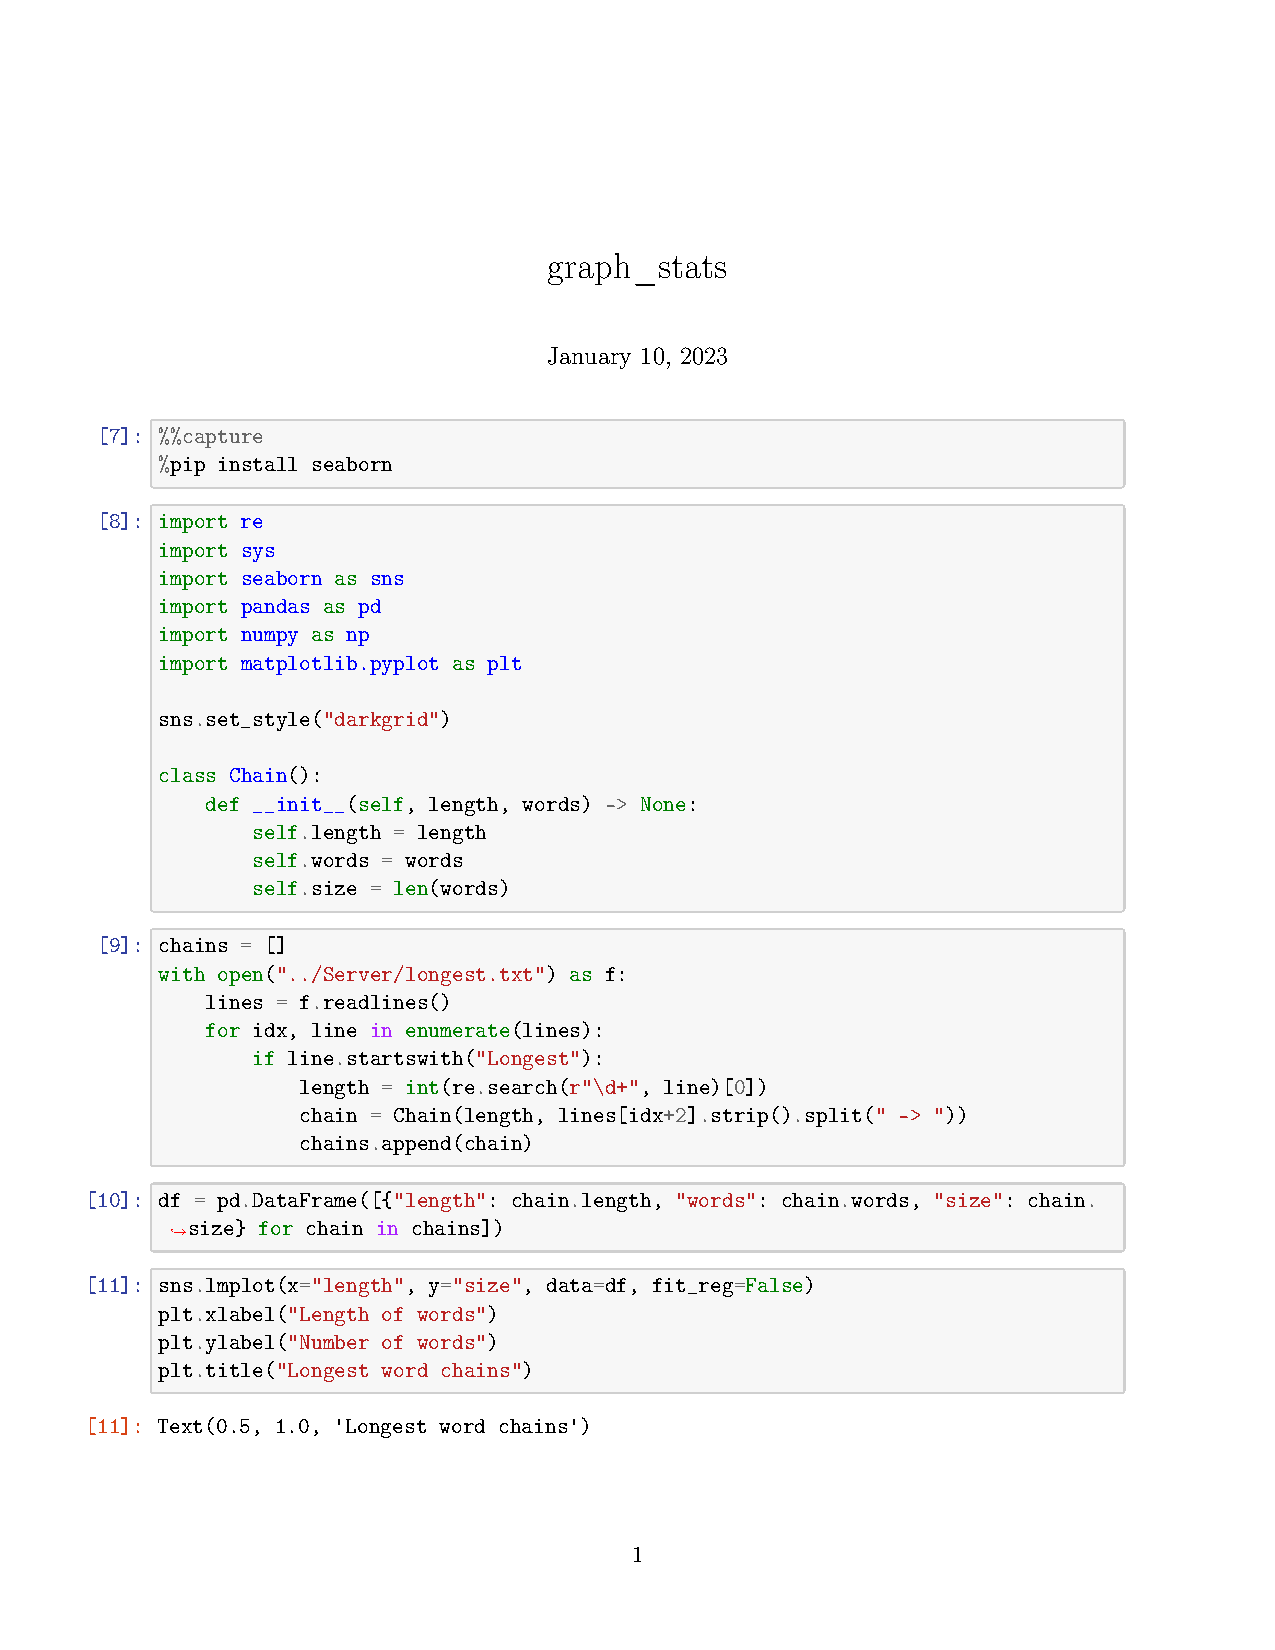
\includepdf[pages=-, offset=25 -25]{graph_stats.pdf}
	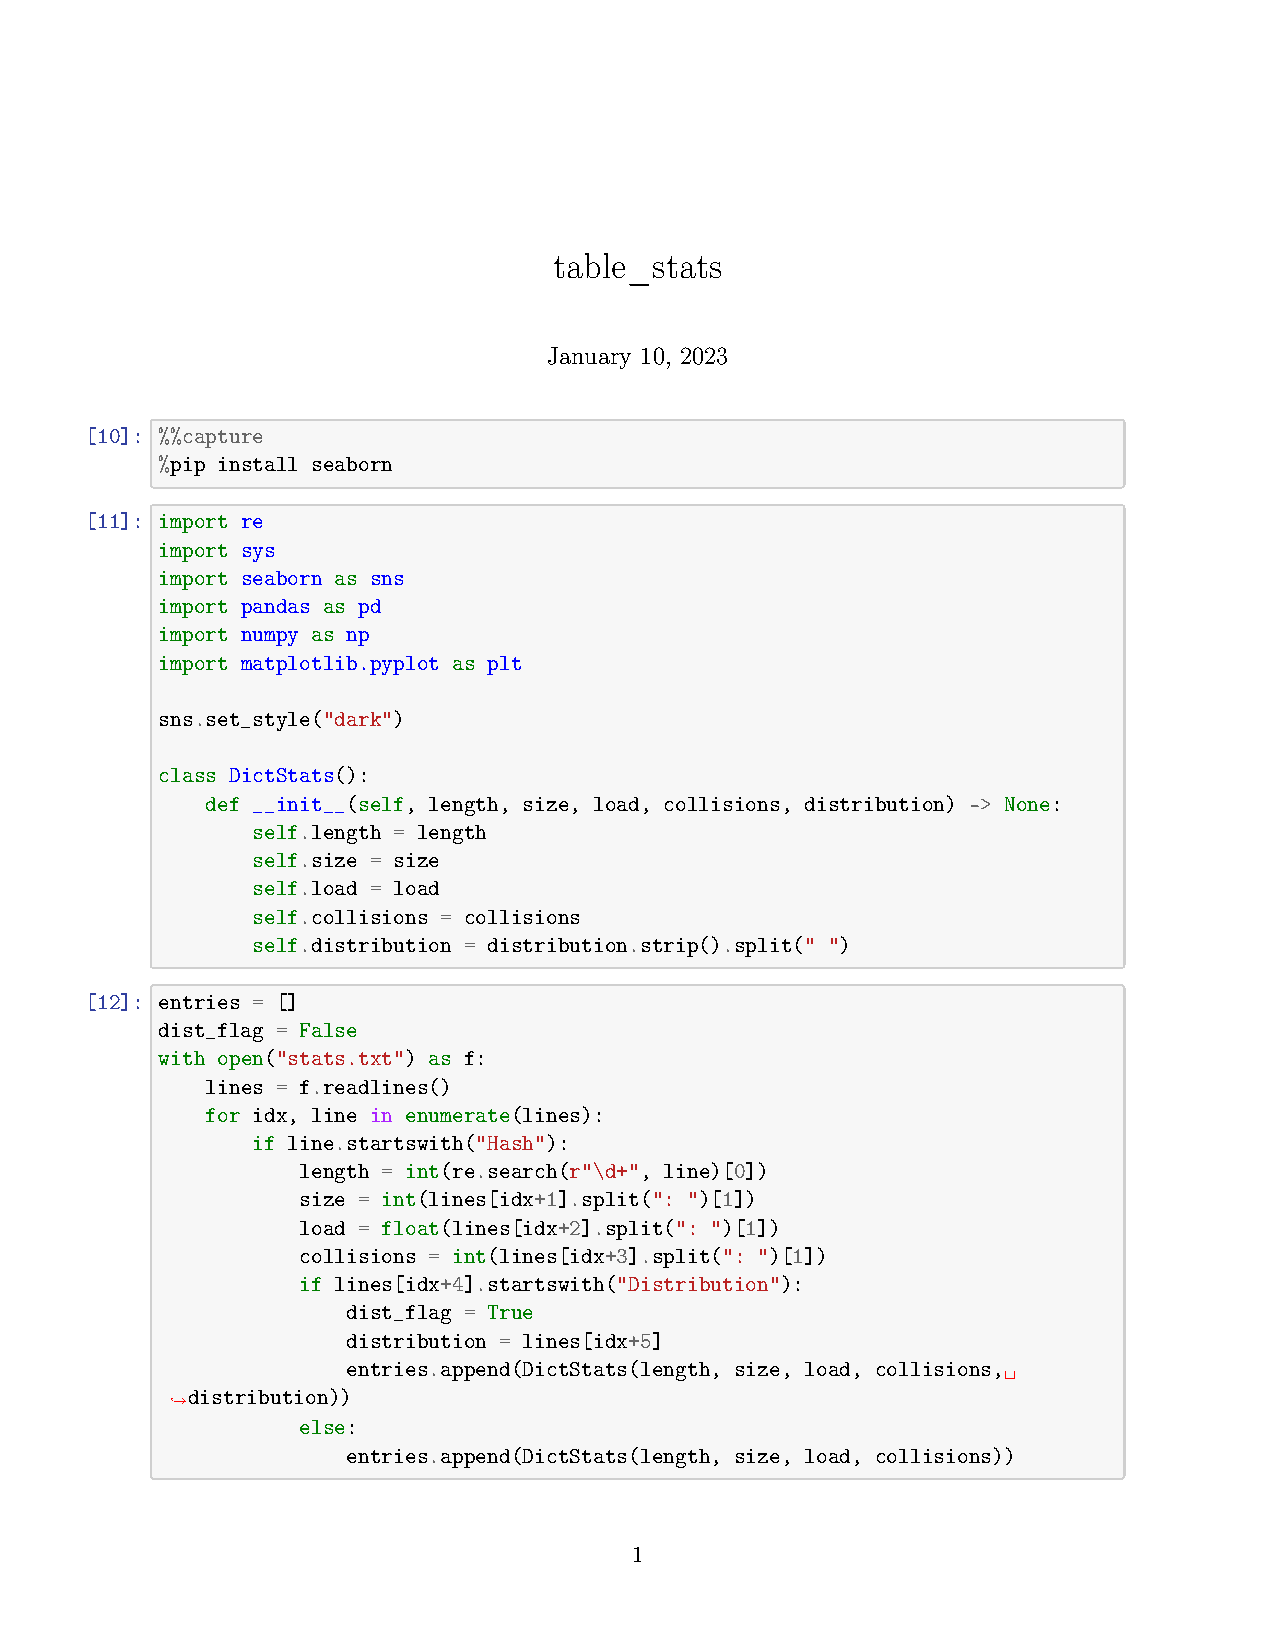
\includepdf[pages=-, offset=25 -25]{table_stats.pdf}
	
\end{document}
